%%\documentclass[12pt,a4paper,spanish]{amsbook}
%%\documentclass[12pt,a4paper,spanish,final,oneside]{iuthesis}
\documentclass[12pt,a4paper,spanish,final,oneside]{iuthesis}
\usepackage[T1]{fontenc}
\usepackage[activeacute,spanish]{babel}
\usepackage[latin1]{inputenc}
\usepackage{graphics}

\makeatletter

\let\SF@@footnote\footnote
\def\footnote{\ifx\protect\@typeset@protect
    \expandafter\SF@@footnote
  \else
    \expandafter\SF@gobble@opt
  \fi
}
\expandafter\def\csname SF@gobble@opt \endcsname{\@ifnextchar[%]
  \SF@gobble@twobracket
  \@gobble
}
\edef\SF@gobble@opt{\noexpand\protect
  \expandafter\noexpand\csname SF@gobble@opt \endcsname}
\def\SF@gobble@twobracket[#1]#2{}
\addto\extrasspanish{\bbl@deactivate{~}}

%%%%%%%%%%%%%%%%%%%%%%%%%%%%%% Textclass specific LaTeX commands.
 \numberwithin{section}{chapter}
 \theoremstyle{plain}
 \newtheorem{thm}{Teorema}[section]
 \numberwithin{equation}{section} %% Comment out for sequentially-numbered
 \numberwithin{figure}{section} %% Comment out for sequentially-numbered
 \theoremstyle{plain}
 \newtheorem{cor}[thm]{Corolario} %%Delete [thm] to re-start numbering
 \theoremstyle{definition}
 \newtheorem{defn}[thm]{Definici\'on}

%%%%%%%%%%%%%%%%%%%%%%%%%%%%%% User specified LaTeX commands.
\usepackage{algorithm}
\usepackage{algorithmic}

\makeatletter

\makeatother
\AtBeginDocument{
  \renewcommand{\labelitemi}{\(\cdot\)}
}

\begin{document}

\title{B�squeda de secuencias repetidas en un modelo de secuenciamiento
aleatorio.}
\author{Cristian S. Rocha (LU 369/96)}

\advisor{Lic. Irene Loiseau}

\degree{Tesis de Licenciatura}
\departmentname{Departamento de Computaci\'{o}n }
\department{Facultad de Ciencias Exactas y Naturales}
\university{Universidad de Buenos Aires}

\submitdate{Agosto de 2002}

\maketitle

{\newpage
\thispagestyle{empty}
\vfill
\vspace*{3cm}

\begin{center}
\bf{Resumen}
\end{center}

El objetivo de esta tesis es proponer una nueva metodolog�a para identificar secuencias repetidas exactas en un conjunto de fragmentos de una secuencia de ADN, y as� permitir el acceso a estos elementos durante su proceso de secuenciamiento aleatorio. 
Surgido de la limitaci�n de conocer el genoma completo del \emph{Trypanosoma cruzi}, para luego as� obtener todas sus repeticiones para su eventual anotaci�n, este trabajo introduce la teor�a de \emph{�lgebra de repeticiones}. Permitiendo as� relacionar correctamente una nueva estructura de datos, $AS^2$, con el problema de encontrar las repeticiones supermaximales de un conjunto de subsecuencias de una secuencia.

\vfill

\begin{center}
\bf{Abstract}
\end{center}

These work introduces a new method to identify exact DNA repeats from a set of fragments of a DNA sequence, to allow queries about them while the random sequence strategy is in progress. 
The limits to know the complete genome of \emph{Trypanosoma cruzi}, do not permit to researchers to annotate all repeats in the known way. In order to solve this problem, these thesis introduces the \emph{repeats algebra} theory to relate a new data structure, $AS^2$, to the \emph{supermaximal repeats in a set of subsequences of a sequence search problem}.

\vspace*{3cm}
 }

{\newpage
\thispagestyle{empty}
\vfill
\vspace*{2cm}

\hfill
\parbox{7cm}{\it Dedico este esfuerzo a la memoria de mi padre; y a mi hermano que fue a probar suerte en otro pa�s.}

\vfill

\begin{center}
{\bf Agradecimientos.}
\end{center}

Antes las eventuales idas y vueltas del desarrollo de esta tesis
me siento comprometido a agradecer a una lista grande de personas
a quienes tengo un gran afecto.


Agradezco a Gabriel Tamburelli, Juan H. Ortega, Maximiliano Sacco y
Alejandro Gomez por su apoyo log�stico. A mi directora de Tesis, 
Irene Loiseau, por la confianza depositada en mi.


Pero el apoyo incondicional otorgado por mi madre, y Gabriela, mi
compa�era de vida, es el fundamento de todo mi trabajo.

\vspace*{5cm}
 }

\tableofcontents
\listoffigures
\listoftables

\chapter{\label{Introduccion}Introducci�n}

\section{\label{Origen}Origen de la Tesis}

A mediados del a�o 1998 se realiz� el primer acercamiento de investigadores del \emph{Instituto de Investigaciones en Ingenier�a Gen�tica y Biolog�a Molecular} (INGEBI) con investigadores del \emph{Departamento de Computaci�n} (DC), ambos pertenecientes de la \emph{Facultad de Ciencias Exactas y Naturales} (FCEN) de la \emph{Universidad de Buenos Aires} (UBA), representados por el Dr. Mariano Levin y la Lic. Irene Loiseau respectivamente. En el mismo, se plante� la posibilidad de construir herramientas computacionales para resolver problemas espec�ficos a tareas de investigaci�n del INGEBI. En este primer acercamiento surgieron problemas de comunicaci�n entre los investigadores de las dos especialidades por el desconocimiento mutuo de los t�rminos usados, por ello se conform� el primer grupo interdisciplinario entre estudiantes, docentes e investigadores de Biolog�a y Computaci�n.

Este grupo tiene como primer objetivo formar especialistas en el campo de la \emph{Biolog�a Computacional}; y luego, pero no menos importante, construir nuevas herramientas para optimizar las tareas de investigaci�n en \emph{Biolog�a Molecular}. Ambos objetivos se est�n llevando a cabo mediante la materia de grado \emph{Introducci�n a la Biolog�a Computacional} que se dicta en el DC, y con la implementaci�n de \emph{la base de datos de secuencias repetidas} del genoma del \emph{Trypanosoma cruzi} , par�sito causante del Mal de Chagas. La misma puede consultarse desde la Internet en la direcci�n http://machi.exp.dc.uba.ar/.

La base de datos se present� como una soluci�n parcial a un problema planteado por el Dr. Levin: {}``clasificar las secuencias repetidas del \emph{T. cruzi}''\footnote{Una repetici�n es una secuencia de s�mbolos que se repite dentro de otra secuencia de s�mbolos. Por ejemplo, la secuencia de s�mbolos del alfabeto {}``issi'' es repetici�n de la secuencia {}``mississippi''. }. Como se ver� con m�s detalle en la secci�n \ref{repeticiones}, las secuencias repetidas, o repeticiones, son clases de secuencias de ADN {}``parecidas'' que se encuentran en un mismo genoma. El INGEBI, como participante del grupo de instituciones involucradas con los proyectos genoma de las especies Trypanos�micas - \emph{Tri-Tryp Consortium} - se comprometi� a especializarse en las repeticiones de los par�sitos que se congregan en el proyecto; para ello debe recolectar, clasificar y crear una nomenclatura clara, sin ambig�edades, para cada repetici�n. A su vez el grupo de Biolog�a Computacional dise�ara las herramientas necesarias para completar este trabajo.

Durante el proceso de maduraci�n del grupo surgieron dos aproximaciones diferentes para encarar el trabajo:

\begin{description}
\item [B�squeda~de~repeticiones~conocidas]El objetivo es encontrar copias de repeticiones previamente estudiadas por m�todos biol�gicos o computacionales.
\item [B�squeda~de~nuevas~repeticiones]El objetivo es encontrar patrones que indiquen la existencia de repeticiones.
\end{description}

Estas aproximaciones no son por completo independientes sino tambi�n complementarias, ya que la primera puede usar a la segunda como entrada de datos. En la figura \ref{Approachs} se puede observar la interacci�n entre los procesos de b�squeda de repeticiones, conocidas y nuevas. Aunque este fue el primer dise�o para encarar el proyecto propuesto por el Dr. Levin, se decidi� por uno que acompa�e el proceso de secuenciamiento del \emph{T. cruzi}, ver secci�n \ref{Proyectos Genomas}. Es por eso que actualmente se esta desarrollando el modelo descripto en la figura\ref{NewApproach}.

\begin{figure}
{\centering 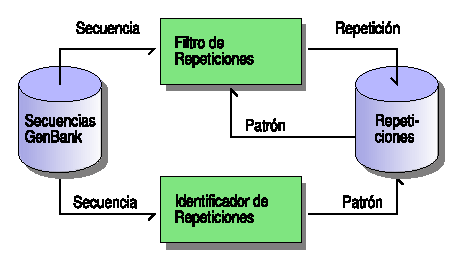
\includegraphics{Approachs.eps} \par}
\caption[Interacci�n entre programas de b�squeda de repeticiones conocidas y de desconocidas.]{\label{Approachs}Interacci�n entre programas de b�squeda de repeticiones conocidas y de desconocidas. Los datos para buscar y encontrar las nuevas secuencias provienen de una \emph{Base de Datos de Secuencias de ADN} (GenBank por ejemplo) y se las procesa para encontrar los patrones conocidos. Los mismos son almacenados en la \emph{Base de Datos de Repeticiones} para luego ser usados por el programa de b�squeda de repeticiones existentes.}
\end{figure}

\begin{figure}
{\centering \resizebox*{1\columnwidth}{!}{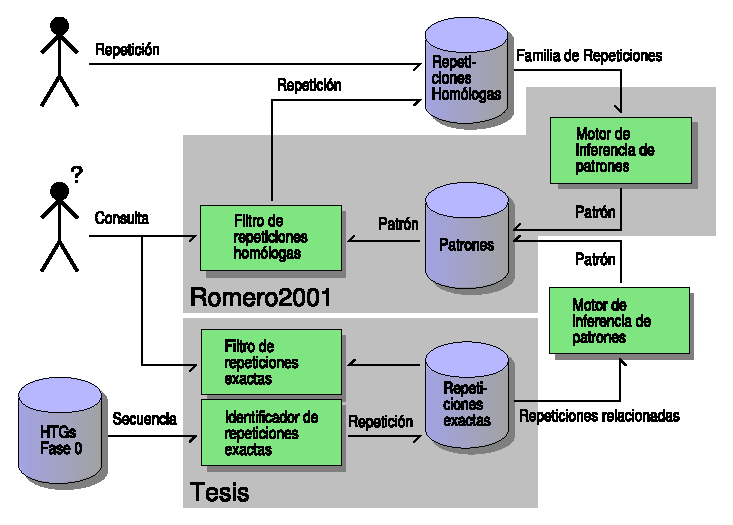
\includegraphics{RealApproachs.eps}} \par}
\caption[Nueva aproximaci�n de la Base de Datos Activa.]{\label{NewApproach}Nueva aproximaci�n de la Base de Datos Activa. Existen dos sistemas interactuando para la b�squeda de repeticiones. El primero basado en t�cnicas de aprendizaje autom�tico puede reconocer estructuras complejas de estructuras de ADN (Romero2001, ver \cite{Romero2001}). El segundo sistema, basado en t�cnicas de combinatoria, recoge la informaci�n de una base de datos HTGs (High Throughput Genomic sequences - Secuencias gen�micas obtenidas con procesos de alto rendimiento) en fase 0 (ver \emph{The HTG GenBank Division}, http://www.ncbi.nlm.nih.gov/HTGS/) para ser procesadas en b�squeda de nuevas repeticiones exactas (Tesis). El motor de inferencia de patrones de repeticiones exactas es un modulo es una tarea pendiente del grupo interdisciplinario.}
\end{figure}

El problema principal que se encontr� a la hora de encarar la b�squeda de las copias dentro de fragmentos es la necesidad de modelar la repetici�n, concepto biol�gico difuso, y es por ello que se encar� la primera aproximaci�n con t�cnicas de aprendizaje autom�tico descripto en \cite{Romero2001}. En la figura \ref{Approachs} se muestra en gris oscuro en que parte del proyecto esta involucrado este trabajo.

Por el otro lado, en esta tesis se encara el problema de buscar nuevas repeticiones, pero no de la manera cl�sica: repeticiones de un fragmento. El autor plantea buscar repeticiones en un conjunto de fragmentos obtenidos aleatoriamente de una secuencia mayor: el genoma, cromosoma o fragmento. Es as� que la tesis cumple con el requisito de buscar repeticiones exactas dentro de una base de datos generada a trav�s de un secuenciamiento aleatorio. La figura \ref{NewApproach} muestra en color gris claro los temas involucrados en esta tesis.

El trabajo esta dividido en cuatro cap�tulos: la presente introducci�n al problema de las repeticiones, como se encara este problema en la actualidad, la estructura de datos propuesta: �rbol de sufijos de supermaximales $AS^2$, y los resultados y conclusiones pertinentes.

\begin{description}
\item [Introducci�n]La secci�n \ref{Otros Fundamentos}, complementa los fundamentos de este trabajo, abarcando otros puntos de inter�s m�s all� del proyecto genoma del \emph{T. cruzi}. En la siguiente, secci�n \ref{Proyectos Genomas}, se explica como las repeticiones influyen en los proyectos genomas en general. Se compara cada aproximaci�n a los proyectos genomas en la secci�n \ref{Secuenciamiento Ordenado vs Aleatorio}. En la secci�n \ref{repeticiones} se presenta la definici�n biol�gica de las repeticiones para luego empezar a describir el problema computacionalmente. La secci�n \ref{Previas} introduce a conceptos que ser�n usados en los pr�ximos cap�tulos.
\item [Estado~del~arte]Este cap�tulo detalla las diferentes aproximaciones que existen en la b�squeda de repeticiones. Se intenta asociar cada aproximaci�n al problema propuesto para luego concluir en la necesidad de construir un modelo que represente mejor el problema. Para finalizar la se presenta las formas de encarar este problema, secci�n \ref{Trabajos Relacionados} y el modelo de supermaximales dado en \cite{Gus97}, secci�n \ref{Modelo de Gusfield de repeticiones}, que ser� la base de nuestro trabajo.
\item [Propuesta]Describe la teor�a para demostrar que el algoritmo es correcto. Primero plantea el problema formalmente, secci�n \ref{Repeticiones en un modelos de secuenciamiento aleatorio}; luego propone un �lgebra de repeticiones para describir que es una repetici�n supermaximal en �ste problema, secci�n \ref{Algebra de Repeticiones}. Se asocia el comportamiento de un �rbol de Sufijos de Supermaximales con el �lgebra de Repeticiones para demostrar que es una estructura v�lida para representar nuestro problema, secci�n \ref{Arbol de Sufijos de Supermaximales}, y se determina los algoritmos para manejar la estructura, secci�n \ref{Algoritmos}.
\item [Resultados~y~conclusiones] En este �ltimo cap�tulo se presentan detalles que se tuvieron en cuenta en la implementaci�n del $AS^2$, secci�n \ref{Implementacion}. Se describe en la secci�n \ref{Resultados} diferentes resultados obtenidos de aplicar el algoritmos sobre genomas que han y est�n siendo secuenciando con t�cnicas aleatorias. Por �ltimo, puede encontrarse las conclusiones de este trabajo en la secci�n.
\ref{Conclusiones}.
\end{description}

\section{\label{Otros Fundamentos}Otros Fundamentos.}

Se ha comparado al Proyecto Genoma Humano con los proyectos m�s ambiciosos de la humanidad: la llegada a la luna o la construcci�n de las pir�mides. La cantidad de recursos que se necesita para poder alcanzar el objetivo es abrumador, y a pesar de ello el mundo cient�fico esta convencido de su utilidad m�dica y tecnol�gica, mas all� del car�cter filos�fico que pueda tener. Tanto es as� que el Proyecto Genoma Humano, completado cinco a�os antes de lo previsto \cite{NCBINfw200}, ahora se extiende a miles de proyectos genomas que van desde virus hasta mam�feros, incluyendo especies ya extinguidas \cite{NCBINs1999}.

Pero aun as� existen problemas muy dif�ciles de abordar, incluso teniendo a disposici�n tantos recursos. Dentro de �stos est�n los inducidos por las \emph{repeticiones}. Tal es as� que un genoma tan importante para Sudam�rica como el del \emph{Trypanosoma cruzi} se ha interrumpido por la gran cantidad y diversidad de estos elementos\cite{MR1999,RMTC99}. Esto da pie a la necesidad de su estudio dando un nuevo punto de vista. Esta tesis aborda el problema de buscar estos elementos en un conjunto de fragmentos, y para ello plantea un nuevo modelo de repeticiones. Esto no quiere decir que es la �nica forma de buscar repeticiones que se conoce, sino que intenta establecer su b�squeda en un campo de batalla en que no se ha intentado antes: durante el proceso de secuenciaci�n.  
Los algoritmos conocidos y las t�cnicas biol�gicas intentan encontrar estos elementos en el genoma completo o directamente sobre la mol�cula de ADN, respectivamente. Pero esto produce contradicciones insalvables: �C�mo buscar repeticiones en el genoma completo si estas mismas repeticiones no nos permite completarlo? �C�mo podemos leer una secuencia repetida de un ADN cuando �sta es m�s larga de lo que nos permite las t�cnicas de secuenciado?

Buscar las repeticiones durante el proceso de una secuenciaci�n aleatoria permite no caer nuevamente en las contradicciones anteriores. La aleatoriedad nos asegura la completa secuenciaci�n de genoma en forma de fragmentos, y por lo tanto no habr� que esperar al ensamblado para conocer estos elementos. Pero igual existe una pregunta que no parece tener una soluci�n obvia. �Se puede ensamblar una secuencia repetida a partir de sus fragmentos? No es objetivo de esta tesis responder esta pregunta pero no se puede hablar de b�squeda de repeticiones en fragmentos sin haberla planteado. Esta tesis conf�a en la afirmaci�n de la respuesta, con lo que se espera que un trabajo a futuro pueda solucionar este problema.

Como se ver� m�s adelante se podr�n encontrar todas las repeticiones maximales en un conjunto de fragmentos obtenidos sin un orden espec�fico.  Hay que notar que aunque no se tiene la respuesta al problema de secuenciar un genoma con grandes cantidades de repeticiones, este trabajo propone un nuevo camino que puede ser el primer paso a la soluci�n tan esperada.

\section{\label{Proyectos Genomas}Proyectos Genomas}

Los Proyectos Genoma tienen como objetivo obtener informaci�n gen�mica de una especie para su eventual estudio. La misma esta almacenada en el \emph{ADN}, macro-mol�culas capaces de guardar toda la informaci�n evolutiva, estructural y funcional de todas las c�lulas que componen a un individuo. Las mismas est�n estructuradas por dos cadenas de nucle�tidos, una inversa-complemento de la otra, formando una doble h�lice. Para este trabajo el concepto b�sico que usaremos es que el ADN puede leerse por fragmentos gracias al proceso denominado \emph{secuenciaci�n}. \cite{Attwood1999}

Simplificando de manera informativa, completar un proyecto genoma necesita de una continua realizaci�n de tareas de secuenciaci�n, ensamblado y anotaci�n. La \emph{secuenciaci�n} es un procedimiento anal�tico para obtener el orden de los nucle�tidos de un ADN\footnote{Este procedimiento no se limita �nicamente a cadenas de nucle�tidos, sino tambi�n a cadenas de amino�cidos. Pero nuestro objetivo es trabajar con nucle�tidos, ya que las repeticiones en cadenas de amino�cidos tienen implicancias completamente diferentes que est�n fuera del alcance de la tesis.} \cite{IUPACCompendium}, o de un punto de vista computacional es la tarea de traducir el DNA en informaci�n digital, o computacionalmente tratable. La informaci�n obtenida es una secuencia de s�mbolos (A, C, G, T); cada uno representa a uno de los cuatro \emph{nucle�tidos}: adenina, citosina, guanina y timina -tambi�n conocidos como \emph{bases}-. Esta tarea est� limitada t�cnicamente a la obtenci�n de secuencias de 400 a 700 s�mbolos de largo. Comparado con el genoma de una especie de \( 5 \cdot 10^{11} \) \emph{pares de bases} (pb) de largo, es casi insignificante lo que se puede realizar en una sola lectura, apenas un \( 1,4 \cdot 10^{-7} \)\% del mismo. Por eso existe la tarea de \emph{ensamblado}; que se encarga de \emph{clasificar}, \emph{ordenar} y \emph{concatenar} los fragmentos con el objetivo de obtener la secuencia completa. La \emph{notaci�n}, en cambio, intenta dar \emph{sintaxis} y \emph{sem�ntica} al genoma \cite{NCBIm2001}.

Las secuencias de 400 a 700 pb, nombradas anteriormente, se las conoce como fragmentos ya que son una parte del DNA y se obtiene por medio de m�todos de \emph{fragmentaci�n} y \emph{clonaci�n}.

Todas las tareas est�n estrechamente relacionadas, por ende un problema con cualquiera de �stas puede inducir al fracaso del proyecto. �Pero qu� problemas podemos encontrar durante todo este proceso?

\begin{description}

\item [\emph{Secuenciamiento}]El principal problema del secuenciamiento es la estructura natural del DNA. Existen diferentes estructuras que promueven su plegamiento obstruyendo la lectura. Este problema se resuelve usando diferentes \emph{geles}\footnote{Los geles son materiales bioqu�micos en donde se sumerge el DNA para ser secuenciado.} como soporte del secuenciado. Pero no existe una �nica soluci�n, con lo que puede ocurrir que para cada fragmento sea necesario cambiar de gel. Estas regiones se las reconoce por tener alto contenido de G-C (Guanina y Citosina), ser pal�ndromos\footnote{Seg�n la Real Academia Espa�ola: palabra o frase que se lee igual de izquierda a derecha, que de derecha a izquierda; p. ej., \emph{anilina}, \emph{d�bale arroz a la zorra el abad}.\\En bioqu�mica: una secuencia de DNA que es igual a su inversa-complemento, por ejemplo: \emph{ACTGCAGT}.} o homopolim�ricas\footnote{Secuencias donde predomina un nucle�tido.}. Un segundo problema, pero de menor medida, es secuenciar regiones no deseadas. La secuenciaci�n involucra un proceso previo de preparaci�n de los fragmentos. Estos se los selecciona de una \emph{biblioteca}, conjunto de fragmentos seleccionados para el secuenciamiento. Cada fragmento esta contenido en un \emph{vector} o \emph{BAC}: soporte para realizar el proceso de clonado necesario para la secuenciaci�n. El problema es que el vector tambi�n es DNA, por lo tanto se puede leer tanto informaci�n del soporte como del fragmento. Este problema se resuelve filtrando las secuencias correspondientes al vector. Luego podemos encontrar los problemas cl�sicos de error por limitaciones t�cnicas de los m�todos usados.\cite{Attwood1999,Roach1998}

\item [\emph{Ensamblado}]\label{Ensamblado} A diferencia de la secuenciaci�n, los problemas no son bioqu�micos sino l�gicos. A partir de una base de datos depurada\footnote{Bases de datos de secuencias que fueron tratadas para eliminar regiones no deseadas: baja calidad de nucle�tidos, vectores y errores.\\Se la puede encontrar en la bibliograf�a como {}``base de datos curadas'', ya se lo ha traducido literalmente del ingles {}``curated databases''. La traducci�n elegida, \emph{base de datos depurada}, expresa mejor el concepto.} donde ya se han resuelto los problemas de la secuenciaci�n se deben obtener la secuencia completa del genoma. Para ellos se va construyendo fragmentos m�s grandes, combinando tareas de clasificaci�n y ensamblado. La \emph{clasificaci�n} tiene como objetivo identificar las secuencias que corresponden a una misma regi�n para obtener una \emph{secuencia consenso} que la represente.\\El \emph{ensamblado} tiene como objetivo poder concatenar estas secuencias consenso; la secuencia obtenida se la conoce como \emph{contig}.\\Cuando trabajamos con repeticiones con largos mayores al l�mite de los que nos proporcionan los secuenciadores (~700 pb) o repeticiones en los extremos de los consensos, nos encontramos con falsas clasificaciones y ambig�edades en el armado de contigs respectivamente. Un cluster es falso si se toma secuencias que corresponden a diferentes regiones del genoma como de una misma regi�n (Ver figura \ref{Figure:FalsoCluster}). Y las ambig�edades se produce por no determinar de forma univoca como ordenar los contigs que contienen una repetici�n en sus extremos (Ver figura \ref{Figure:Ambiguedad}).\cite{NCBIm2001,Roach1998,BorkCopley2001}

\begin{figure}
{\centering \resizebox*{1\columnwidth}{!}{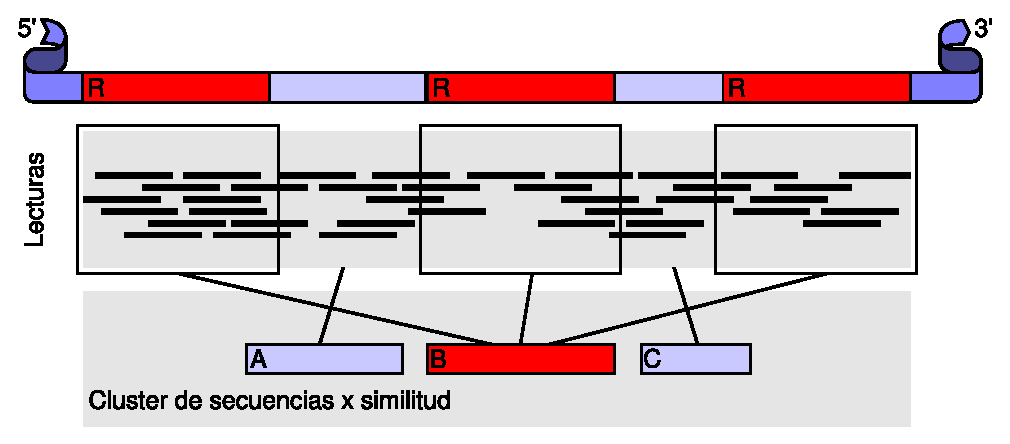
\includegraphics{FalsoCluster.eps}} \par}
\caption[Esquema de generaci�n de un cluster falso.]{\label{Figure:FalsoCluster}Esquema de generaci�n de un cluster falso. La figura representa cinco regiones, tres de ellas, \emph{R}, son copias de una misma repetici�n. Relacionando las lecturas por similitud, se obtienen tres clusters. El cluster \emph{B} unifica las tres regiones correspondientes a la repetici�n \emph{R}, por lo tanto esta configuraci�n de contigs es falsa.}
\end{figure}

\begin{figure}
{\centering \resizebox*{1\columnwidth}{!}{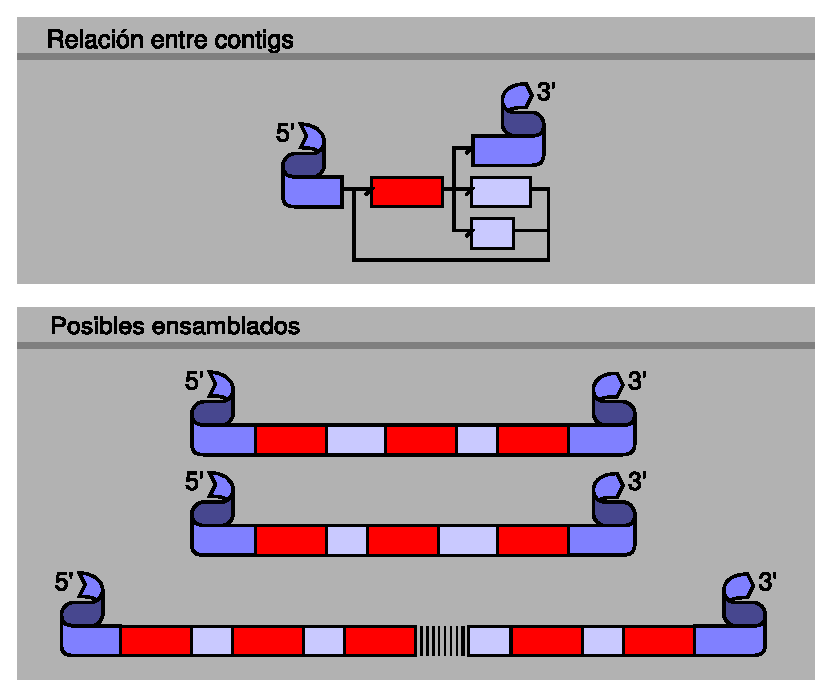
\includegraphics{Ambiguedad.eps}} \par}
\caption[Esquema de ambig�edad.]{\label{Figure:Ambiguedad}Esquema de ambig�edad. A partir de la figura \ref{Figure:FalsoCluster} se tienen cinco clusters. Si se intenta ordenas estos clusters se tiene infinitas soluciones posibles si desconocemos que los clusters de azul claro no son repeticiones. En el caso que sabemos que no lo son, existen solo dos formas de ordenar los clusters.}
\end{figure}

\item [\emph{Anotaci�n}]Existen diversas complicaciones a la hora de plasmar las conclusiones o investigaciones en una regi�n exacta del genoma y todo se debe a la complejidad del modelo tratado. Por ejemplo, actualmente las bases de datos gen�micas almacenan miles de \emph{prote�nas hipot�ticas} provocando entre los investigadores diferentes interpretaciones \cite{Russo00,Ashburner00}. La imposibilidad de clasificar e identificar cada elemento del genoma de manera un�voca a enviciado a publicar resultados obtenidos computacionalmente, muchas de ellas con t�cnicas heur�sticas, como verdades absolutas. Y esto ocurre por la desinformaci�n sobre estas t�cnicas, sumado a que todav�a el genoma es un laberinto oscuro, declarar a las herramientas computacionales como funcionalmente v�lidas es dejar pistas falsas en la interpretaci�n del genoma.\cite{Roach1998,NCBIm2001}
\end{description}

Como se puede observar, hemos hecho hincapi� en las repeticiones. Esto no implica que las repeticiones son la �nica fuente de problemas, pero si de su gran mayor�a, y puede encontrarse en cada etapa del proceso de un proyecto genoma.

\section{\label{Secuenciamiento Ordenado vs Aleatorio}Secuenciamiento Ordenado vs. Aleatorio.}

Existen dos tipos b�sicos de \emph{secuenciamientos} para encarar proyectos genoma: \emph{ordenado} y \emph{aleatorio}. Ambas pueden complementarse para completar un proyecto genoma ya que cada uno tiene virtudes y defectos contrapuestos.

\begin{description}
\item [Caminado]La primera t�cnica se basa en la existencia de primers. Un \emph{primer} es una secuencia �nica dentro de una regi�n o fragmento del genoma y sirve para marcar el comienzo del secuenciamiento. El proceso de \emph{caminado} conlleva una continua b�squeda de primers y secuenciaci�n de fragmentos adyacentes ( Ver figura \ref{Figure:Caminado}. Aunque es te�ricamente sencilla la tarea es ardua y consume una cantidad muy alta de recursos, adem�s de estar condenada a tiempos imposibles cuando los genomas son medianos o grandes, ya que cada paso puede durar d�as. Se usa en regiones peque�as y para resolver un ensamblado\cite{DEO,Roach1998}

\begin{figure}
{\centering \resizebox*{1\columnwidth}{!}{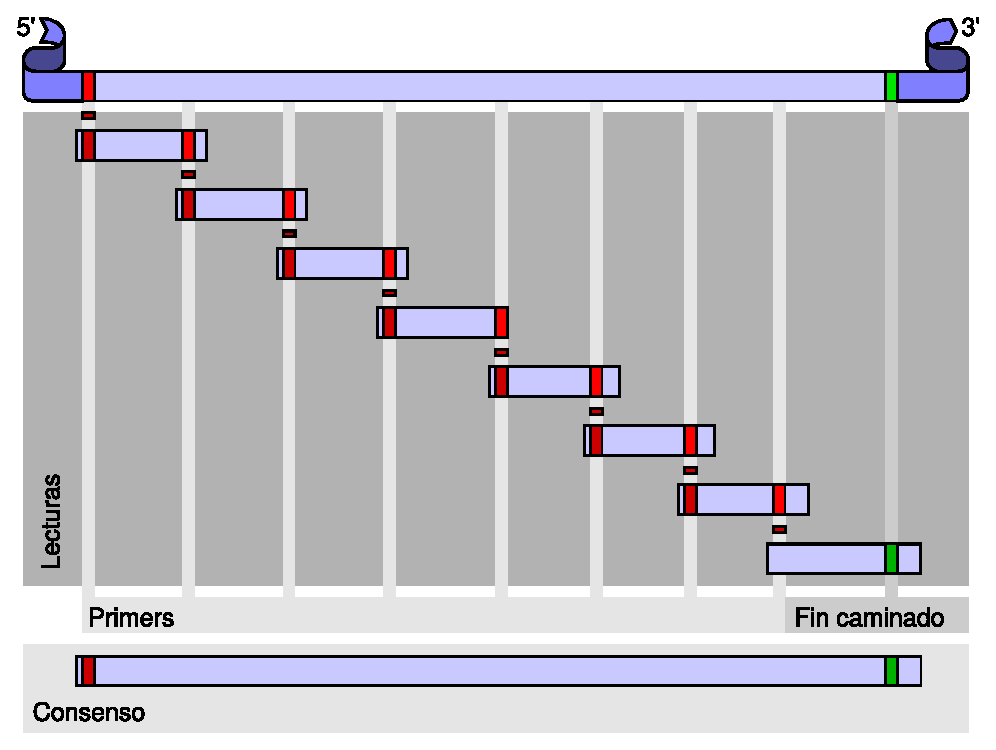
\includegraphics{Caminado.eps}} \par}
\caption[Secuenciamiento ordenado.]{\label{Figure:Caminado}Secuenciamiento ordenado. El proceso de caminado se realiza a partir de un \emph{primer} inicial que indica el principio de la regi�n del genoma a secuenciar. Luego se realizar lecturas sucesivas a partir de los nuevos primers que se valla {}``recolectando'' en el camino.}
\end{figure}

\item [Shotgun]El \emph{secuenciamiento aleatorio}, o \emph{shotgun}, empieza fragmentando una parte, o todo el genoma en un conjunto de piezas al azar de longitudes conocidas. Esto nos permite realizar secuenciamiento en paralelo con lo que se acelera dr�sticamente el procesamiento ( Ver figura \ref{Figure:Shotgun} ). A�n as� el ensamblado termina siendo un proceso m�s complejo, aunque automatizable. Para resolver los problema de espacios no secuenciados (\emph{GAPs}) o \emph{subsecuenciados}, ver figura \ref{Figure:RegionesSubsecuenciadas}, se asegura que la cantidad de lecturas sobre la regi�n a secuenciar sean suficientes gracias a los estudios estad�sticos de Landerman. Si esta estad�stica no satisface, que es posible, se completa el secuenciamiento con la t�cnica de caminado. \cite{DEO,Roach1998}.

\begin{figure}
{\centering \resizebox*{10cm}{!}{\includegraphics{Shotgun.eps}} \par}
\caption[Secuenciamiento aleatorio.]{\label{Figure:Shotgun}Secuenciamiento aleatorio. Los procesos de secuenciamiento \emph{shotgun} fragmentan el genoma de manera aleatoria, para luego leer todos los fragmentos para ensamblarlos. Si la t�cnica fragmenta todo el genoma aleatoriamente se la conoce como \emph{Whole Genome Shotgun}, WGS. En caso de que la fragmentaci�n sea por cromosoma se lo conoce como \emph{Whole Chromosome Shotgun}, WCS. Otras t�cnicas fragmentan el cromosoma a partir de marcas, \emph{BAC ends}, que luego se usan para ordenar los fragmentos una vez que se ensamblen a partir de un secuenciamiento aleatorio. Esta estrategia se la conoce como 'Map-as-you-go'.}
\end{figure}

\begin{figure}
{\centering \resizebox*{1\columnwidth}{!}{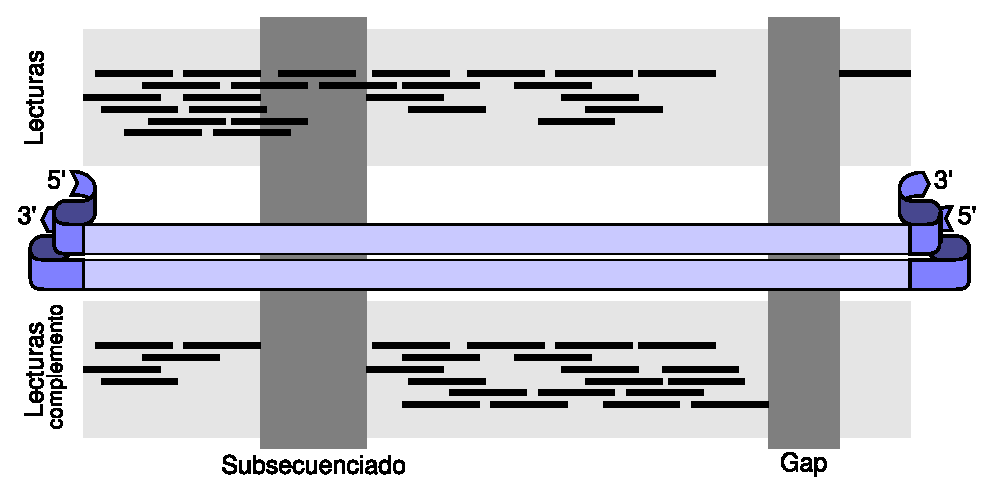
\includegraphics{RegionesSubsecuenciadas.eps}} \par}
\caption[Esquema de regiones subsecuenciadas.]{\label{Figure:RegionesSubsecuenciadas}Esquema de regiones subsecuenciadas. En este gr�fico se presenta una regi�n que fue secuenciada de forma aleatoria. Los fragmentos superiores fueron secuenciados de 5' a 3', mientras que los inferiores fueron secuenciados de 5' a 3', su complementario. Se describe en la figura dos regiones, una que tiene un espacio no secuenciado (GAP) y otro subsecuenciado al cual falta secuenciar la hebra complementaria (Hebra simple).}
\end{figure}

\end{description}

\label{Cobertura}El n�mero en promedio en que un nucle�tido esta representado por una base de alta calidad en una colecci�n de secuencias obtenidas aleatoriamente se lo conoce como \emph{cobertura}. En otras palabras, la cobertura es la relaci�n entre la cantidad de nucle�tidos que debemos leer y la cantidad de nucle�tidos que compone nuestro fragmento a secuenciar ( Ver figura \ref{Figure:Cobertura} ). Una simple f�rmula descripta en \cite{Lander88}, puede estimar la cobertura necesaria para secuenciar aleatoriamente una parte del genoma para prevenir los problemas del ensamblado. El cuadro \ref{tab: Cobertura} muestra valores usados para aproximar la cobertura. Por ejemplo si se obtiene 100.000 \emph{pares de bases} (pb) de un clon de 100 Kpb, se espera haber secuenciado el 63\% del clon, ya que 100.000 es una ves (1x) la cantidad de pb del clon. Por lo tanto es muy com�n ver que la mayoria de los genomas son secuenciados bajo una cobertura de entre 8x y 10x.

\begin{figure}
{\centering \resizebox*{1\columnwidth}{!}{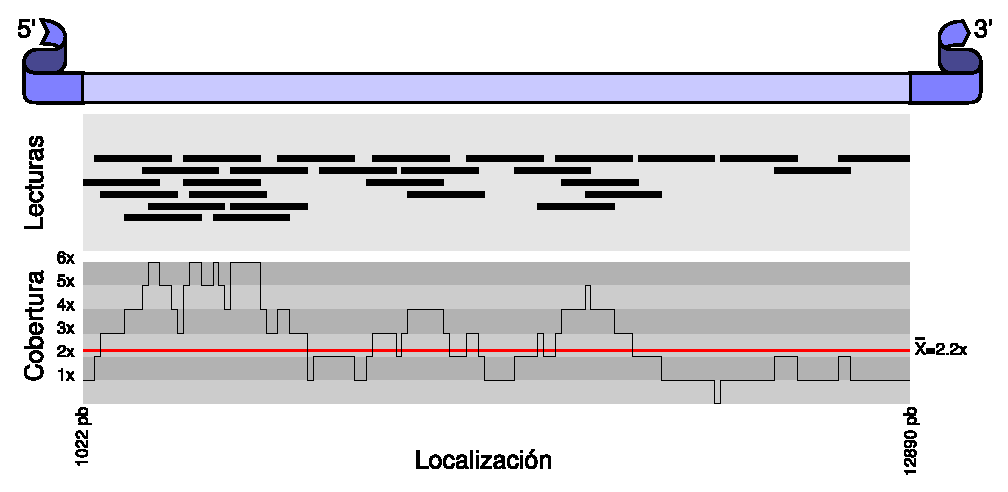
\includegraphics{Cobertura.eps}} \par}
\caption[Esquema de cobertura.]{\label{Figure:Cobertura}Esquema de cobertura. En la figura se representa un regi�n del genoma que fue secuenciada aleatoriamente. El gr�fico inferior describe, nucle�tido a nucle�tido, la cobertura correspondiente. La cobertura media es de $2.2x$.}
\end{figure}

\begin{table}
\begin{tabular}{|c|c|}
\hline
Cobertura&Porcentaje del clon secuenciado\\
\hline
\hline
0,25x&22\%\\
\hline
0,50x&39\%\\
\hline
0,75x&53\%\\
\hline
1x&63\%\\
\hline
2x&88\%\\
\hline
3x&95\%\\
\hline
4x&98\%\\
\hline
5x&99,4\%\\
\hline
6x&99,75\%\\
\hline
7x&99,91\%\\
\hline
8x&99,97\%\\
\hline
9x&99,99\%\\
\hline
10x&99,995\%\\
\hline
\end{tabular}
\vspace{.5cm}

\caption{\label{tab: Cobertura}Relaci�n entre la cobertura y el porcentaje
del clon secuenciado.}
\end{table}

\section{\label{repeticiones}Secuencias repetidas}

En \cite{MGA} se describe la organizaci�n del genoma en dos tipos de elementos, \emph{genes de copia �nica} y \emph{DNA repetitivo}. Este �ltimo a su vez organizado en diferentes subclases, ver figura \ref{Figure:Repeticiones}. 

\begin{figure}
{\centering \resizebox*{1\columnwidth}{!}{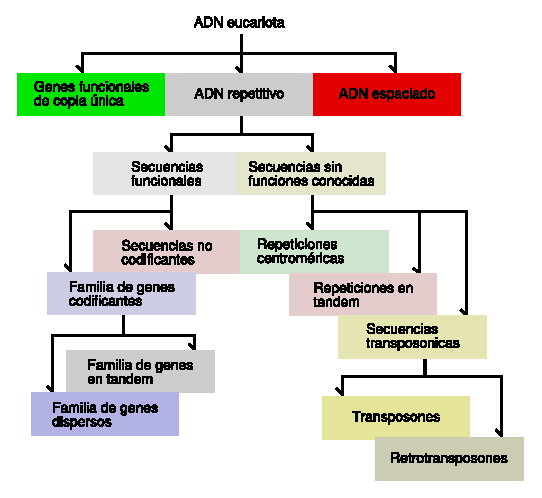
\includegraphics{Repeticiones.eps}} \par}
\caption[Organizaci�n de las mol�culas de ADN eucariota.]{\label{Figure:Repeticiones}Organizaci�n de las mol�culas de ADN eucariota. (ver \cite{MGA})}
\end{figure}

\begin{description}
\item [Repeticiones~funcionales]Algunas funciones gen�ticas se presentan en m�ltiples copias. Todas ellas pertenecen a alguna de estas clases.
\begin{description}
\item [Familia~de~genes~dispersos]Muchas genes que codifican en prote�nas se agrupan en familias por homolog�a. Genes de una misma familia pueden tener leves diferencias a�n cumpliendo la misma funci�n. Aunque existen casos en que las funciones pueden diferir.
\item [Arreglos~de~familia~de~genes~en~t�ndem]Una manera de satisfacer las necesidades de la c�lula de gran cantidad de productos de algunos genes es organizar los mismos en t�ndem. O sea, m�ltiples copias adyacentes de un mismo gen.
\item [Secuencias~que~no~codifican]Los tel�meros son una regi�n del genoma que contiene secuencias que no codifican, no obstante estas regiones son de vital importancia para la estabilidad del cromosoma. Estos se componen de una gran cantidad de copias de secuencias muy cortas de DNA organizadas en t�ndem.
\end{description}
\item [Repeticiones~sin~funci�n~conocida]Las repeticiones que no tengan funcionamiento conocido se las organizan de la siguiente manera.
\begin{description}
\item [DNA~altamente~repetitivo~del~centr�mero]Se puede encontrar una gran cantidad de repeticiones, organizados en t�ndem, que flaquean el centr�mero de los cromosomas.
\item [VNTR]Son una clase especial de repeticiones en t�ndem de entre 15 y 100 nucle�tidos. Se encuentran dispersos por todo el genoma.
\item [Transposones]Una gran proporci�n del genoma eucariota est�n compuestos de elementos que son capaces de propagarse. A trav�s de un proceso de copia estas secuencias llamadas transposones puede reubicarse en otras regiones. Si las secuencias que se insertan en el genoma provienen de un RNA, se los conoce como retrotransposones.
\end{description}
\end{description}

A partir de esta descripci�n de las repeticiones podemos llegar a caracterizar atributos comunes a las repeticiones: largo, cantidad, conservaci�n y dispersi�n. El \emph{largo} y la \emph{cantidad} son atributos triviales, y no as� el resto que pasaremos a detallar.

\begin{description}
\item [Conservaci�n]Las copias pueden variar levemente entre ellas. Las diferencias son las que determina el \emph{grado de conservaci�n}. Este atributo puede variar dentro de la secuencia de manera tal de identificar regiones con menos cambios que otras. Se puede ver esta complejidad en la estructura en familias de genes, como es el caso de VIPER ( Ver figura \ref{Figure:Viper} ) en el \emph{T. cruzi} o la familia de genes que codifican la hemoglobina en el humano ( Ver figura \ref{Figure:Hemoglobina} ). En cambio las VNTRs son muy conservadas.

\begin{figure}
{\centering \resizebox*{1\columnwidth}{!}{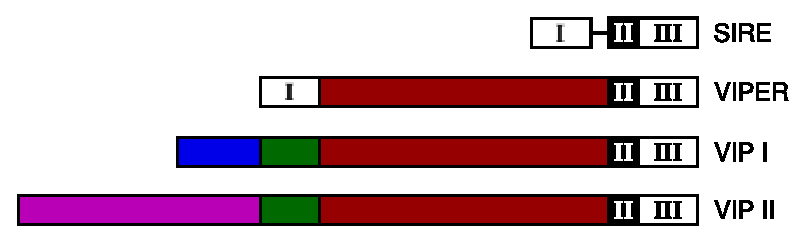
\includegraphics{Viper.eps}} \par}
\caption[Organizaci�n de VIPER.]{\label{Figure:Viper}Organizaci�n de VIPER, retroelemento relacionado con retrotransposones LTR, ver \cite{Vazquez2000}.}
\end{figure}

\begin{figure}
{\centering \resizebox*{6cm}{!}{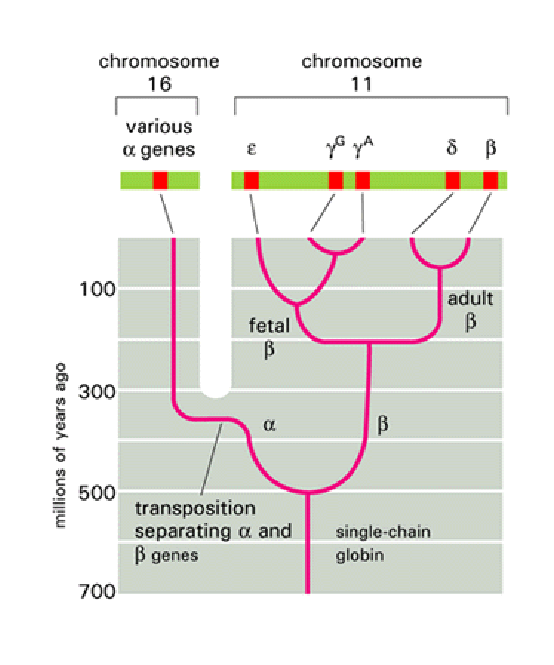
\includegraphics{Hemoglobina.eps}} \par}
\caption[Organizaci�n de la hemoglobina.]{\label{Figure:Hemoglobina}Evoluci\'{o}n de la familia de genes de la hemoglobina en el genoma humano.}
\end{figure}

\item [Dispersi�n]Indica como se distribuyen las copias en el genoma. Puede ser \emph{local} a una regi�n bien definida, como es el caso de las repeticiones centrom�ricas o telom�ricas. Como tambi�n se las puede encontrar \emph{dispersas} como los transposones.

\end{description}

\section{\label{Previas}Previas.}

Antes de comenzar a describir m�s el problema, es necesario realizar varias aclaraciones sobre la notaci�n usada en el texto. En principio los t�rminos \emph{s�mbolo}, \emph{letra} y \emph{car�cter} se entender�n como sin�nimos, refiri�ndose a la entidad m�nima de lo que est�n compuesto las secuencias. As� tambi�n se ver�n intercalados los t�rminos \emph{secuencia, palabra} y \emph{cadena} para referencia a una sucesi�n ordenada de esta entidad m�nima. En cambio, \emph{fragmento} y \emph{subsecuencia} son conceptos diferentes. Un fragmento, como se ha dicho, es una secuencia de DNA o prote�na que ha sido obtenido por m�todos de clonaci�n o cortando una secuencia mayor. A diferencia de fragmento, subsecuencia es una referencia a una regi�n de una secuencia. La misma no tiene sentido si no hay una secuencia que la contenga.

Desde el punto de vista biol�gico un elemento repetido es una clase de fragmentos hom�logos dentro de un mismo genoma. Pero la definici�n de \emph{repetici�n} en una \emph{cadena de s�mbolos} no es tan amplia ya que se toma el concepto de igualdad estructural y no de homolog�a para identificarlas. En consecuencia se usa el concepto de similaridad, que aunque es una aproximaci�n a la homolog�a da excelentes resultados.


\chapter{\label{Estado del arte}Estado del arte}

Lo que no se ha encontrado durante el proceso de investigaci�n de esta tesis es informaci�n o art�culos sobre la obtenci�n o estad�stica de estos elementos durante el proceso de secuenciamiento. La totalidad de las referencias involucran el genoma completo \cite{Roach1998}, por lo que cualquier estudio es v�lido si se completa el secuenciamiento. Es por eso que la totalidad de las referencias de algoritmos encontradas tienen como precondici�n una �nica secuencia de donde se busca las repeticiones.

\section{\label{Trabajos Relacionados}Trabajos relacionados.}

Adem�s de los art�culos relacionados con la b�squeda exacta de repeticiones en una cadena de caracteres, existe un n�mero considerable de escritos que se especializan en la detecci�n de repeticiones degeneradas \footnote{En la literatura sobre cadena de caracteres se conoce a las repeticiones degeneradas como repeticiones aproximadas o inexactas. }. En general los m�todos se dividen en dos grupos.\cite{kurtz00computation}

\begin{description}
\item [M�todos~exactos]Se basan en la formalizaci�n de un modelo de repetici�n, y luego
localizan todas las regiones en una secuencia que cumplen con la definici�n. \cite{Fitch86,Leung91,Benson94,Kannan96,Schmidt98,Benson99,Landau01,marsan00algorithms}
\item [M�todos~heur�sticos]No pueden garantizar encontrar todas las repeticiones bajo cualquier modelo espec�fico.\cite{BensonWaterman94,Agarwal94,Rivals97,Vincens98,Benson99,Babenko99}
\end{description}

Tampoco se ha encontrado referencias al problema de encontrar repeticiones en una colecci�n de fragmentos de secuencias gen�micas. No as�, en cambio, sobre optimizaci�n de b�squedas de sufijos y prefijos de secuencias en base de datos en general\cite{jagadish00effective}, que en su objetivo de optimizar la consulta utilizan �ndices de subcadenas en com�n siendo referencias importantes para resolver el problema. Entonces se propone dividir, nuevamente, este tipos de problemas de b�squeda de repeticiones en:

\begin{description}
\item [�nica~secuencia]La mayor�a de los trabajan bajo este paradigma ya que se esfuerzan en buscar repeticiones en una regi�n.
\item [Conjunto~de~secuencias]Existen trabajos relacionados como el caso de los �rboles de sufijos generalizados ( ver secci�n \ref{ASG} ), pero el objetivo en general es buscar palabras en textos, pero no se ha encontrado un uso gen�mico para este algoritmo.
\end{description}

A�n as�, para describir mejor el objetivo de esta tesis hay que incluir una nueva clasificaci�n para b�squedas de repeticiones en un conjunto de secuencias.

\begin{description}
\item [Secuencias~independientes]Las secuencias del conjunto de entrada no est�n superpuestas. Todos los algoritmos existentes trabajan bajo esta suposici�n.
\item [Secuencias~dependiente]Las secuencias son subsecuencias de una misma secuencia y est�n superpuestas. Llamaremos \emph{cobertura} a la cantidad de veces que una posici�n de la secuencia mayor se encuentra representada en las subsecuencias. Por ejemplo, la mayor cobertura del conjunto \( { abcc, yuab, ccak, uab } \) de la secuencia $\alpha = yuabccak$ es de $3x$, ya que $ab$ se encuentra 3 veces en $\alpha$. La menor cobertura es de $1x$, ya que $k$ solo se encuentra una �nica vez en el conjunto. La cobertura promedio se calcula s�mbolo a s�mbolo, por lo que en promedio $\alpha$ tiene una cobertura de $1.875x$. No se ha encontrado trabajos previos.
\end{description}

Bajo esta clasificaci�n, esta tesis se concentra en la \emph{b�squeda de repeticiones exactas en un conjunto de secuencias dependientes}. Para justificar la elecci�n de repeticiones exactas debemos responder la siguiente pregunta: �Qu� tan similar es una secuencia a otra? Existen varios modelos de distancia que tienen en cuenta mutaciones, equivalencia entre nucle�tidos, llegando a ser probabil�sticamente complejos. A�n as�, tomando cualquiera de estas forma para medir la similitud, no se puede asegurar que dos secuencias similares correspondan a dos fragmentos hom�logos. Bas�ndose en �ste hecho se puede suponer que la igualdad entre secuencias es una buena aproximaci�n al concepto de homolog�a, por ello en el resto de la tesis solo se hablar� de igualdad entre secuencias para identificar elementos repetidos. Esta afirmaci�n no quita valor a las normas de similitud existentes, solo simplifica el problema que interesa tratar para poder, a futuro, plantear un modelo m�s complejo.

\section{\label{Modelo de Gusfield de repeticiones}Modelo de Gusfield de
repeticiones}

Un problema a la hora de identificar secuencias repetidas es determinar cuando una secuencias es repetida, o mejor dicho, cuando una repetici�n es importante. En principio la secuencia vac�a es repetici�n para cualquier cadena de cualquier lenguaje, por lo tanto es una repetici�n trivial y no se tendr�n en cuenta. Otras repeticiones triviales son las de largo uno, los s�mbolos. Tambi�n se incluyen todas las subsecuencias de una secuencia repetida y as� se tiene una cantidad desorbitante de soluciones sin valor informativo. En pos de definirlas de manera tal que las soluciones sean significativas se ha incluido el concepto de \emph{maximal} dando las siguientes definiciones\cite{Gus97}.

\begin{defn}
Un \emph{par maximal} (o un par de repetici�n maximal) en una cadena \( S \) es un par de subcadenas id�nticas \( \alpha \) y \( \beta \) en \( S \) tal que el car�cter inmediatamente posterior (anterior) de \( \alpha \) es diferente al car�cter posterior (anterior) de \( \beta \). De otra manera, si extendemos \( \alpha \) y \( \beta \) en ambas direcciones dejan de ser iguales. Un par maximal esta representado por una tupla \( <p_{1},p_{2},n\prime > \), donde \( p_{1} \) y \( p_{2} \) indican la posici�n de inicio en ambas subcadenas y \( n\prime \) indica el largo. Para una cadena \( S \) definimos \( R(S) \) como el conjunto de todos los pares maximales de \( S \).
\end{defn}

Eligiendo la secuencia \( S=xabcyiiizabcqabcyrxar \), se encuentran tres ocurrencias de la secuencia \( abc \). La primera y la segunda ocurrencia conforman el primer par maximal \( <2,10,3> \). La segunda con la tercera conforman el par \( <10,14,3> \). Pero no es par maximal la primera con la tercera ocurrencia. En cambio, si se toma la secuencia \( abcy \) se obtiene que sus dos �nicas ocurrencias son el par maximal \( <2,14,4> \). Ahora, si la secuencia es \( cxxaxxaxxb \) observamos un par maximal solapado correspondiente a la secuencia \( xxaxx \). Notar que este caso es permitido por la definici�n.

Ahora, en algunos casos es �til conseguir todas los pares maximales de una secuencia, en otros casos la cantidad de soluciones puede ser inmanejable, por lo tanto ser�a �til definir un concepto m�s restringido.

\begin{defn}
Una \emph{repetici�n maximal} \( \alpha \) es una subcadena de \( S \) que corresponde a un par maximal de \( S \). En otros t�rminos, \( \alpha \) es una repetici�n maximal en \( S \) si hay una tupla \( <p_{1},p_{2},|\alpha |>\in R(S) \) y \( \alpha \) aparece en las posiciones \( p_{1} \) y \( p_{2} \) en \( S \). Diremos que \( R\prime (S) \) es el conjunto de repeticiones maximales de \( S \).
\end{defn}

Del ejemplo anterior con la secuencia \( S \) donde ambas cadenas \( abc \) y \( abcy \) son repeticiones maximales, se puede observar que la cantidad de pares es mayor que la cantidad de repeticiones. Esto ocurre porque cada cadena esta representado por lo menos un par maximal, entonces concluimos que \( |R(S)|>|R\prime (S)| \). En general la cantidad de \( |R\prime (S)| \) va a ser muy inferior que \( |R(S)| \) por lo que, aunque este conjunto es m\'{a}s modesto, da una idea clara de la soluci�n al problema.

Ahora, existen casos en que la definici�n de repetici�n maximal no es suficiente. Tomando una nueva secuencia \( S=a\alpha bx\alpha ya\alpha b \). Aqu� la subcadena \( \alpha \) es un repetici�n maximal como lo es tambi�n \( a\alpha b \), la cual es supersecuencia de \( \alpha \). Quiz�s no se desea reportar secuencias \( \alpha \) como repetici�n ya que existe una repetici�n maximal que la contiene que puede ser m�s informativa.

\begin{defn}
Una \emph{repetici�n supermaximal} es una repetici�n maximal que no es subcadena de otra repetici�n maximal.
\end{defn}

Para Gusfield, las repeticiones maximales y supermaximales y los pares maximales son las �nicas tres maneras v�lidas para definir estructuras �tiles de repeticiones exactas. Esta afirmaci�n solo es v�lida en el modelo de buscar repeticiones en una �nica secuencia, a continuaci�n se plantear� los mismos conceptos para un conjunto de secuencias.

\subsection{\label{MGG}Modelo de Gusfield generalizado.}

Tomemos ahora un conjunto de secuencias \( S \). Para cada secuencia \( s \in S \) podemos usar las misma definiciones de par maximal, repetici�n maximal, y repetici�n supermaximal, pero no ocurre lo mismo para un conjunto de secuencias ya que lo que para una secuencia no es repetida para \( s \) puede que lo sea para un conjunto si es compartida por otra secuencia. Para ello generalizaremos las definiciones de par maximal, repetici�n maximal y supermaximal para un conjunto de secuencias. Previamente se definir� a \( \alpha (\pi ,\sigma ) \) como la subsecuencia de \( \alpha \) que comienza en la posici�n \( \pi \) y termina en \( \sigma \). Y \( S_{\tau } \) es la secuencia identificada con \( \tau \) en el conjunto de secuencias \( S \).

\begin{defn}
Un \emph{par maximal} es un par de subsecuencia id�nticas \( \alpha \) y \( \beta \) de secuencias existentes en \( S \) las cuales dejan de ser iguales si se las extiende en ambos lados.

Un par maximal del conjunto \( S \) se representa por la tupla \( <id_{a},id_{b},p_{a},p_{b},n\prime >_{S} \), donde \( id_{a} \) y \( id_{b} \) son la identificaci�n de las secuencias en \( S \), \( p_{a} \) y \( p_{b} \) son la ubicaci�n de la repetici�n en la secuencia $S$ y \( n\prime \) es el largo. Para un conjunto \( S \) definimos \( R(S) \) como el conjunto de todas las tuplas maximales de \( S \).

\begin{eqnarray*}
R(S) & = & \{<id_{a},id_{b},p_{a},p_{b},n\prime >|\\
(id_{a} & \neq & id_{b}\vee p_{a}\neq p_{b})\wedge \\
S_{id_{a}}\left( p_{a},p_{a}+l\right) & = & S_{id_{b}}\left( p_{b},p_{b}+n\prime \right) \wedge \\
S_{id_{a}}\left( p_{a},p_{a}+n\prime +1\right) & \neq & S_{id_{b}}\left( p_{b},p_{b}+n\prime +1\right) \wedge \\
S_{id_{a}}\left( p_{a}-1,p_{a}+n\prime \right) & \neq & S_{id_{b}}\left( p_{b}-1,p_{b}+n\prime \right) \}
\end{eqnarray*}

\end{defn}

A partir del del conjunto de secuencias \( S=\{ \)\( xabclop, \) \( lapabx, \) \( pabcjabp\} \) se concluye: la secuencia \( ab \) corresponde para los siguientes pares maximales \( <1,2,2,4,2> \), \( <1,3,2,6,2> \), \( <2,3,4,2,2> \), \( <2,3,4,6,2> \) y \( <3,3,2,4,2> \). Obs�rvese que la definici�n nos permite realizar pares con la misma secuencia, incluyendo de esta manera la definici�n de par maximal para una �nica secuencia. Para el caso de la secuencia \( abc \) se tiene �nicamente el par \( <1,3,2,2,3> \).

\begin{defn}
Una secuencia \( \alpha \) es \emph{repetici�n maximal} de un conjunto \( S \) si existe un par maximal que corresponda a \( \alpha \). En si, \( \alpha \) es una repetici�n maximal en \( S \) si hay una tupla \( \left\langle i_{a},i_{b},p_{a},p_{b},|\alpha |\right\rangle \in R(S) \) y \( \alpha \) aparece en las posiciones \( p_{a} \) en la secuencia \( i_{a} \) y \( p_{b} \) en la secuencia \( i_{b} \) del conjunto \( S \). Diremos que \( R\prime (S) \) es el conjunto de repeticiones maximales de \( S \). \[ R\prime (S)=\{\alpha \in \Delta ^{*}|(<i_{a},i_{b},p_{a},p_{b},l>\in R(S))(S_{i_{b}}\left( p_{b},p_{b}+l\right) =\alpha )\}\] 
\end{defn}

Entonces, tomando el mismo ejemplo anterior, las secuencias \( ab \) y \( abc \) pertenecen a \( R'(S) \). Nuevamente se concluye que el conjunto \( R\prime (S) \) es inferior que \( R(S) \), por corresponder a cada secuencia en \( R'(S) \) por lo menos una tupla en \( R(S) \). De la misma manera vamos reduciendo la respuesta, pero todav�a se puede tener una soluci�n demasiado abultada para tratarla f�cilmente. La pr�xima definici�n limita m�s la respuesta, de igual manera en que lo hac�a el modelo de Gusfield.

\begin{defn}
Una repetici�n \emph{supermaximal} es una repetici�n maximal que no es subcadena de otra repetici�n maximal. Llamaremos \( M(S) \) al conjunto de las repeticiones supermaximales.\[ M(S)=\left\{ \alpha \in R'(S)\left| \left( \exists \beta ,\gamma \in \Delta ^{*}\right) \left( \beta \alpha \gamma \neq \alpha \wedge \beta \alpha \gamma \in R\acute{'}(S)\right) \right. \right\} \] En este caso, podemos ver que \( abc \) es repetici�n supermaximal y no as� \( ab \). As� se obtiene un conjunto m�s peque�o, con lo que se espera que sea mucho m�s tratable.
\end{defn}

\subsection{�rboles de sufijos para la b�squeda de repeticiones en una secuencia.}

Los �rboles de sufijos\cite{Weiner73,McCreight76,Ukkonen95} y arreglo de sufijos\cite{Manber93} son estructuras de datos que facilitan la b�squeda de cadenas. Gusfield realiza una detallada discusi�n sobre estos elementos en \cite{Gus97}. Como el arreglo de sufijos es una interpretaci�n del �rbol de sufijos sobre un arreglo, solo se discutir� �nicamente sobre los �rboles de sufijos. 

En principio, estos �rboles de sufijos tienen una gran potencia ya que permiten diferentes tipos de consultas sobre los elementos que se encuentran almacenados en la estructura. La necesidad de explicar esta estructura es que es la base del algoritmo propuesto para resolver el problema. En si, Gusfield propone un algoritmo sobre la b�squeda de repeticiones sobre un �rbol de sufijos dando las definiciones previamente explicadas, pero en esta nueva aproximaci�n no se desarrolla un �rbol de sufijo de una secuencia sino de las secuencias supermaximales de un conjunto de secuencias.

Los �rboles de sufijos de una secuencia \( \alpha \) son �rboles, parecidos a los Trie\cite{Fredkin60} o PATRICIA\cite{Mirrison68}, cuyas ramas corresponden a un sufijo%
\footnote{Si \( \alpha =a_{1}a_{2}a_{3}\ldots a_{n-2}a_{n-1}a_{n} \), entonces
\( \alpha _{i}=a_{i}a_{i+1}a_{i+2}\ldots a_{n-2}a_{n-1}a_{n} \) es
el sufijo de \( \alpha \) en la posici�n \( i \).

Por ejemplo: para \( \alpha =mississippi \), tenemos los siguientes
sufijos: \( \alpha _{1}=mississippi=\alpha \), \( \alpha _{2}=ississippi \),
\( \alpha _{3}=ssissippi \), \( \alpha _{4}=sissippi \), \( \alpha _{5}=issippi \),
\( \alpha _{6}=ssippi \), \( \alpha _{7}=sippi \), \( \alpha _{8}=ippi \),
\( \alpha _{9}=ppi \), \( \alpha _{10}=pi \), \( \alpha _{11}=i \),
\( \alpha _{11}=i \), \( \alpha _{12}=\lambda \).
} de \( \alpha \). Por ejemplo, sea la secuencia \( \alpha =xabcyiiizabcqabcyrxar \).
En la figura \ref{Figure:ArbolSufijo.}
\begin{figure}
\resizebox*{3in}{4in}{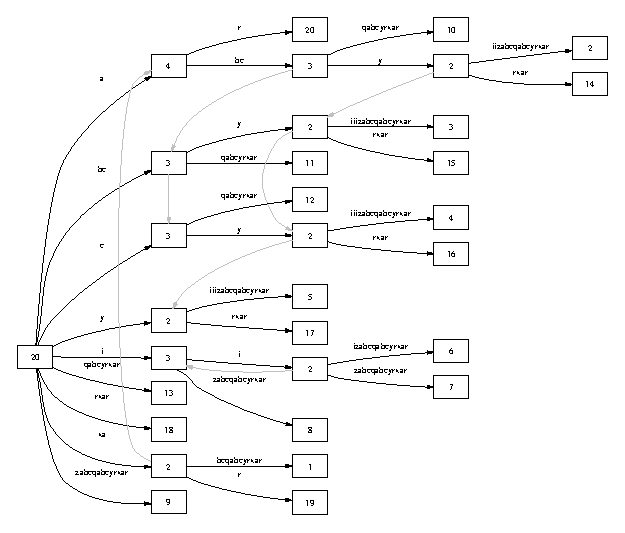
\includegraphics{suffixtree.eps}}

\caption{\label{Figure:ArbolSufijo.}�rbol de sufijos para {}``xabcyiiizabcqabcyrxar''.}
\end{figure}
 vemos el �rbol de sufijo para \( \alpha \). Si recorremos el �rbol desde la ra�z, en profundidad, vamos a recorrer las ramas que corresponden a los sufijos de \( \alpha \).

Un �rbol de sufijos puede ser usado para buscar una subcadena de largo \( m \) en tiempo \( O(m) \). Como existen \( n(n+1)/2 \) subcadenas en una secuencia \( \alpha \) de largo \( n \) no queda claro como es posible construir el �rbol en un tiempo \( O(n) \). Agregando solo un car�cter a la secuencia \( \alpha \), se tienen \( n+1 \) nuevas secuencias, pero ellas no son independientes. Weiner (1973) dio el primer algoritmo y Mc. Creight (1976) dio una mejor aproximaci�n para la construcci�n de �rboles de sufijos cuando se procesa a \( \alpha \) de derecha a izquierda. Solo m�s tarde Ukkonen (1992, 1995) dio un algoritmo linean procesando la secuencia de izquierda a derecha. 

\subsection{\label{ASG}�rbol de sufijos generalizado}

El �rbol de sufijos que es capaz de almacenar una colecci�n de palabras se lo conoce como \emph{ASG}. Tiene las mismas propiedades que el �rbol de sufijo para una sola secuencia, pero se diferencian por la etiqueta usada en cada uno de los ejes del �rbol. Mientras que el primero almacena una colecci�n de referencias a la secuencia y subsecuencia relacionada con el eje del �rbol, el segundo solo almacena colecci�n de subsecuencia. Como se ve, el �rbol com�n es un �rbol generalizado con una �nica referencia a la misma secuencia.

Gusfield propone en \cite{Gus97} dos algoritmos de orden lineal que encuentran todas repeticiones maximales y supermaximales. Este modelo conlleva tener un �rbol de sufijos armado en donde se realiza la b�squeda. Luego proponen una compactaci�n del �rbol dejando solo las ramas donde intervienen repeticiones. Como podremos observar en el cap�tulo \ref{Modelo} vamos a intercalar estas nociones con ventajas relacionadas a la t�cnica de secuenciamiento aleatoria.

\section{\label{El problema de encontrar...}Repeticiones en el secuenciamiento.}

Como se ha dicho, en un modelo aleatorio, las secuencias se obtienen de regiones aleatorias del genoma. Durante este proceso las secuencias se van almacenando en una base de datos. Esta base de datos se las conoce como base de datos de primera pasada, ya que no han sido clasificadas%
\footnote{Las secuencias se clasifican por regi�n a las que pertenecen, t�cnicas usadas para la clasificaci�n y otros datos seg�n corresponda a la especie estudiada y la t�cnica usada. } ni filtradas%
\footnote{Las secuencias se filtran de repeticiones conocidas y de basura que correspondan al vector usado para secuenciar. }. Una vez revisadas, las secuencias pasan a una base de datos depurada. Este proceso termina cuando se obtenga la cobertura predeterminada \ref{Cobertura}.

�Qu� ocurre con las repeticiones durante todo este proceso? Si la repetici�n es conocida es eliminada para que no provoque ambig�edades en el proceso de ensamblado. En el caso contrario se ver� que existe grandes ambig�edades y falsos clusters en el ensamblado. Lo ideal es no llegar al ensamblado con repeticiones.

Existe un problema innato que hace no f�cil el reconocimiento en este modelo. Una cobertura de 10x implica que necesitamos haber le�do cada nucle�tido en promedio 10 veces. Entonces podemos esperar que una regi�n va a tener por lo menos 10 lecturas. Es una conclusi�n directa suponer que si existe una repetici�n \( \alpha \), por haber sido le�da 10 veces al final del procedimiento, debe encontrarse en el conjunto de las secuencias obtenidas m�s que esta cantidad. Si existen dos copias de una repetici�n, entonces deben existir $c$ lecturas de cada una, donde $c$ es la cobertura dada para el genoma $G$. Por lo tanto, podemos asegurar que si una secuencia se repite m�s de $2 \dot c$ veces es una repetici�n en $G$.

\vspace{1cm}
\fbox{ \parbox{10cm}{\textbf{Problema:} Se busca encontrar repeticiones supermaximales en una colecci�n de secuencias independientes bajo una cobertura de $2c$, donde $c$ es la cobertura con la que se ha secuenciado la regi�n del genoma.} }


\chapter{\label{Modelo}Repeticiones en un conjunto de secuencias dependientes}

\section{\label{Repeticiones en un modelos de secuenciamiento aleatorio}Repeticiones en un modelo de secuenciamiento aleatorio}

Como hemos planteado, nuestra preocupaci�n es obtener secuencias repetidas en t�cnicas de secuenciamiento shotgun, y de la misma ha surgido las siguiente inc�gnita:

Si estamos obteniendo secuencias aleatoriamente, podemos concluir que podemos secuenciar varias veces la misma regi�n, es m�s, se espera tener secuenciado al menos \( c \)x todos las bases del genoma al termino del secuenciamiento \ref{Cobertura}. A la vez las secuencias repetidas tienen m�s de una copia dentro del genoma. Entonces �C�mo saber si una secuencia es repetida o es un fragmento varias veces secuenciado? �Qu� ocurre con las repeticiones cuando tenemos en cuenta que estamos en un proceso donde se va obteniendo nuevas secuencias durante todo el proceso?

Una secuencia esta repetida si se puede reconocer entre los fragmentos m�s de \( 2 c \) copias de una repetici�n. Se puede ser m�s espec�fico y decir que, si la cantidad de copias encontradas es de \( 2 n \), entonces deben existir al menos \( \frac{n}{c} \) copias en el genoma. Esta aproximaci�n ingenua asegura detectar todas las repeticiones al final del secuenciamiento, ya que si se encuentra una repetici�n en un fragmento, este no salta a la vista hasta tener la cobertura $c$x en el mismo.

\section{\label{Algebra de Repeticiones}�lgebra de repeticiones.}

Para describir y demostrar la correcci�n del algoritmo que presentaremos debemos introducir nuevas nociones sobre repeticiones que nos ser�n muy �tiles. En su conjunto plantear� una sencilla y nueva �lgebra basada en expresiones regulares y en conjuntos finitos, para luego deducir propiedades sobre repeticiones.

Partiendo del modelo propuesto por Gusfield junto con la generalizaci�n propuesta para buscar repeticiones en un conjunto de secuencias {[}\ref{MGG}{]}, se plantean las siguientes definiciones sobre el conjunto de secuencias \( S \) correspondientes a un alfabeto , donde cada secuencia se identifica un�vocamente por un n�mero entero \( \tau \), y \( S_{\tau } \) es la secuencia. Siendo \( S_{10} \) la secuencia identificada con el n�mero \( 10 \). Una subsecuencia de \( S_{i} \) que comience en la posici�n \( \pi \) y termine en \( \sigma \) la indicaremos como \( S_{i}(\pi ,\sigma ) \). Por ejemplo, si la secuencia \( axfggh \) esta identificada con el n�mero \( 10 \), entonces \( S_{10}(2,5)=xfg \). Si \( \pi \) es mayor o igual a \( \sigma \), \( S_{i}(\pi ,\sigma ) \) da la secuencia vac�a; de igual manera si \( \pi \) o \( \sigma \) est�n fuera del rango de la secuencia \( S_{i} \).

\begin{defn}
La tupla de subsecuencias \( \left\langle i,\pi ,\sigma \right\rangle _{S} \) identifica a la subsecuencia de la secuencia \( i \), que pertenece al conjunto \( S \), que comienza en la posici�n \( \pi \) y termina en la posici�n \( \sigma \).

Una \emph{consulta} sobre una colecci�n de secuencias \( S \) es un conjunto \( Q_{S} \) de tuplas de subsecuencias. Si para toda tupla de la consulta \( Q_{S} \) existe una secuencias \( \alpha \) que le corresponde la tuplas \( \left\langle i,\pi ,\sigma \right\rangle _{S} \) tal que \( S_{i}(\pi ,\sigma )=\alpha \) diremos que la \emph{consulta es v�lida} para el conjunto \( S \). Para extender nuestra definici�n de consulta diremos que \( Q_{S}(\alpha ) \) es el subconjunto de tuplas \( \left\langle i,\pi ,\sigma \right\rangle _{S} \) de \( Q_{S} \) que corresponde a \( S_{i}(\pi ,\sigma )=\alpha \). El largo de la cadena \( \alpha \) la notaremos como \( |\alpha | \).
\end{defn}

Nuestro objetivo es conseguir un \( Q_{S} \) que contenga solo las secuencias supermaximales de \( S \). En otras palabras pedimos que para cada tupla \( \left\langle i,\pi ,\sigma \right\rangle \in Q_{S}(\alpha ) \), consulta v�lida de \( S \), exista una tupla maximal \( <j,j',p,p',|\alpha |>\in R\prime (\alpha ) \) tal que \( j=i \) y \( p=\pi \), � \( j'=i \) y \( p'=\pi \).

Toda esta teor�a supone que este dado de antemano un alfabeto \( \Delta \) al que pertenece todas las palabras del conjunto \( S \). Para simplificar la notaci�n, a partir de ahora supondremos estar hablando de un �nico conjunto \( S \), con lo que no se pondr� los sub�ndices que indican el conjunto, excepto que se indique lo contrario.

\begin{defn}
Si el conjunto \( A \) tiene m�s de \( c \) elementos entonces \( \Phi _{c}A=A \), sino \( \Phi _{c}A=\emptyset \). Esta funci�n \( \Phi _{c} \) la conoceremos como la funci�n \emph{c-repetici�n} sobre conjuntos.

\begin{eqnarray*}
\Phi _{c}S & = & S,\#S>c\\
\Phi _{c}S & = & \emptyset ,\#S\leq c
\end{eqnarray*}

\end{defn}

La funci�n \( \Phi _{c} \) nos permitir� descartar los conjuntos de secuencias que no correspondan a repeticiones. Llamaremos a \( c \) el \emph{grado de repetici�n de la consulta} cuando el conjunto sea una consulta. Tambi�n simplificaremos la notaci�n y no escribiremos el umbral \( c \) mientras no sea necesario, ya que siempre trabajaremos con un umbral fijo.


\subsection{�lgebra de repeticiones.}

Para comenzar con las definiciones, primero vamos a definir el conjunto de repeticiones sobre una secuencia y sobre una expresi�n regular.

\begin{defn}
Un conjunto de repeticiones \( \left( \alpha \right) \) es un conjunto de tuplas \( \left\langle i,\pi ,\sigma \right\rangle \) ( consulta ) donde \( S_{i}\left( \pi ,\sigma \right) =\alpha \) cuando existe m�s de una tupla, y es vaci� si existe una o ninguna tupla.

\begin{equation}
\label{math:rep-seq}
\left( \alpha \right) ^{c}_{S}=\Phi _{c}\left\{ \left\langle i,\pi ,\sigma \right\rangle _{S}\left| S_{i}\left( \pi ,\sigma \right) =\alpha \right. \right\} =\Phi _{c}Q_{S}\left( \alpha \right)
\end{equation}

\end{defn}

Como ejemplo tenemos el conjunto \( S \) de secuencias \( \{tacgua, \) \( agata, \) \( gatca\} \). La consulta \( (ga) \) esta conformado por \( \{\left\langle 2,2,3\right\rangle , \)\( \left\langle 3,1,2\right\rangle \} \) si tomamos las identificaci�n de la secuencia empezando por \( 1 \). Ahora si tomamos la consulta \( (gu) \) es vac�a ya que aunque existe la tupla \( \left\langle 1,3,4\right\rangle \), es �nica por ende \( gu \) no es repetici�n. Una consulta importante, pero trivial, es la correspondiente a la secuencia vac�a \( (\lambda ) \). Esta va a contener un n�mero infinito de tuplas, ya que, como hemos descripto la tuplas cuyos \( \pi \) y \( \sigma \) que est�n fuera de rango de la secuencia, o \( \pi \) menor a \( \sigma \), describen a la secuencia vac�a.

Ahora daremos m�s potencia a este conjunto de secuencias para no solo consultar sobre una secuencia sino que tambi�n sobre expresiones regulares \footnote{Las expresiones regulares las vamos a expresar entre barras '/ ' para diferenciarlas de las cadenas del lenguaje. }. Este tipo de consulta da mayor potencia ya que se puede expresar un conjunto de consultas de secuencias que cumplan con la expresi�n.

\begin{defn}
Un conjunto de repeticiones \( \left( \left/ \beta \right/ \right) \) es una consulta cuyas tuplas \( \left\langle i,\pi ,\sigma \right\rangle \) corresponde a una secuencia repetida que cumple con la expresi�n regular \( \left/ \beta \right/ \) \footnote{\( S_{i}(\pi ,\sigma )\in /\beta / \) }

\begin{equation}
\label{math:rep-exp}
\left( \left/ \beta \right/ \right) ^{c}_{S}=\left\{ \left\langle i,\pi ,\sigma \right\rangle _{S}\in \left( S_{i}\left( \pi ,\sigma \right) \right) ^{c}_{S}\left| S_{i}\left( \pi ,\sigma \right) \in \left/ \beta \right/ \right. \right\}
\end{equation}

\end{defn}

Tomando el ejemplo anterior, la consulta \( \left( \left/ t.*a\right/ \right) \) esta compuesta por las tuplas \( \{\left\langle 1,1,2\right\rangle , \) \( \left\langle 2,4,5\right\rangle \} \), ya que la �nica repetici�n que cumple con la expresi�n regular es \( ta \). Una consulta m�s interesante es \( \left( \left/ .*\right/ \right) \) que contiene las tuplas \( \{\left\langle 1,1,2\right\rangle , \) \( \left\langle 2,4,5\right\rangle , \) \( \left\langle 2,2,3\right\rangle , \) \( \left\langle 3,1,2\right\rangle , \) \( \left\langle 2,2,4\right\rangle , \) \( \left\langle 3,1,3\right\rangle \} \) \( \bigcup \) \( \left( \lambda \right) \) de las repeticiones \( ta \), \( ga \), \( gat \) y la secuencia vac�o. Notar que si hubiera otra repetici�n en el conjunto entonces sus tuplas estar�an en este conjunto. Otra consulta interesante es aquella que no incorpora la secuencia vac�a: \( \left( \left/ .+\right/ \right) \).

Para relacionar ambas definiciones damos el siguiente corolario:

\begin{cor}
\label{corollary:rep-seq-exp}Un conjunto de repeticiones sobre expresiones regulares verifica la siguiente igualdad:

\begin{equation}
\label{math:rep-seq-exp}
\left( \left/ \beta \right/ \right) ^{c}_{S}=\bigcup _{\alpha \in \left/ \beta \right/ }\left( \alpha \right) ^{c}_{S}
\end{equation}

\end{cor}

\begin{proof}
La nueva expresi�n de \( \left( \left/ \beta \right/ \right) \) es otra forma para describir la expresi�n {[}\ref{math:rep-exp}{]}.
\end{proof}

\begin{defn}
La operaci�n \emph{extensi�n} (\( \cdot \)) sobre consultas v�lidas da una nueva consulta v�lida cuyas secuencias son repetidas y extensiones de la consulta original. La extensi�n se realiza a la derecha si el operador se encuentra a la derecha de la notaci�n, o a la izquierda en otro caso.

\begin{eqnarray}
\left( \alpha \right) ^{c}_{S}\cdot & = & \bigcup _{\alpha \in \Delta }\left( \alpha a\right) ^{c}_{S}\label{math:ext} \\
\cdot \left( \alpha \right) ^{c}_{S} & = & \bigcup _{\alpha \in \Delta }\left( a\alpha \right) ^{c}_{S}
\end{eqnarray}

\end{defn}

\begin{cor}
Realizar una extensi�n a derecha (izquierda) a una consulta de una expresi�n regular \( \beta \) equivale a una consulta de expresi�n regular \( \beta \cdot \) (\( \cdot \beta \)).

\begin{eqnarray}
\left( \left/ \beta \right/ \right) ^{c}_{S}\cdot & = & \left( \left/ \beta \cdot \right/ \right) ^{c}_{S}\label{math:exp-reg} \\
\cdot \left( \left/ \beta \right/ \right) ^{c}_{S} & = & \left( \left/ \cdot \beta \right/ \right) ^{c}_{S}
\end{eqnarray}

\end{cor}

\begin{proof}
Comenzando por la expresi�n definici�n \ref{math:ext}, y usando el corolario \ref{corollary:rep-seq-exp}, podemos demostrar la igualdad.

\begin{eqnarray*}
\left( \left/ \beta \right/ \right) _{S}^{c}\cdot & = & \bigcup _{\alpha \in \left/ \beta \right/ }\left( \alpha \right) ^{c}_{S}\cdot \\
 & = & \bigcup _{\alpha \in \left/ \beta \right/ }\left( \bigcup _{a\in \Delta }\left( \alpha a\right) ^{c}_{S}\right) \\
 & = & \bigcup _{\alpha \in \left/ \beta .\right/ }\left( \alpha \right) ^{c}_{S}\\
 & = & \left( \left/ \beta .\right/ \right) ^{c}_{S}
\end{eqnarray*}

\end{proof}

Gracias a estos dos operadores podemos presentar dos nuevos conjuntos que nos ayudaran con una definici�n alternativa de repeticiones maximales, y adem�s de ser el pilar del algoritmo propuesto. Las siguientes definiciones son v�lidas tanto para secuencias como para expresiones regulares ya que se basan en los conceptos definidos previamente.

\begin{defn}
Una \emph{consulta extensible} a la derecha (izquierda) es una consulta cuyas tuplas est�n extendidas a la derecha (izquierda) en la extensi�n de la consulta.

\begin{eqnarray}
\left( \alpha \right\rangle ^{c}_{S} & = & \Phi ^{c}\left\{ \left\langle i,\pi ,\sigma \right\rangle _{S}\in \left( \alpha \right) ^{c}_{S}\left| \left\langle i,\pi ,\sigma +1\right\rangle _{S}\in \left( \alpha \right) ^{c}_{S}\cdot \right. \right\} \label{math:rep-expansible} \\
\left\langle \alpha \right) ^{c}_{S} & = & \Phi ^{c}\left\{ \left\langle i,\pi ,\sigma \right\rangle _{S}\in \left( \alpha \right) ^{c}_{S}\left| \left\langle i,\pi -1,\sigma \right\rangle _{S}\in \cdot \left( \alpha \right) ^{c}_{S}\right. \right\}
\end{eqnarray}

Una \emph{consulta no extensible} a la derecha \emph{}(izquierda) es una consulta cuyas tuplas no est�n extendidas a la derecha (izquierda) en la extensi�n de la consulta.

\begin{eqnarray}
\left( \alpha \right] ^{c}_{S} & = & \Phi ^{c}\left\{ \left\langle i,\pi ,\sigma \right\rangle _{S}\in \left( \alpha \right) ^{c}_{S}\left| \left\langle i,\pi ,\sigma +1\right\rangle _{S}\notin \left( \alpha \right) ^{c}_{S}\cdot \right. \right\} \label{math:rep-noexpansible} \\
\left[ \alpha \right) ^{c}_{S} & = & \Phi ^{c}\left\{ \left\langle i,\pi ,\sigma \right\rangle _{S}\in \left( \alpha \right) ^{c}_{S}\left| \left\langle i,\pi -1,\sigma \right\rangle _{S}\notin \cdot \left( \alpha \right) ^{c}_{S}\right. \right\}
\end{eqnarray}

Una consulta cuyas tuplas est�n en una consulta (no) extensible a derecha y en una consulta (no) extensible a la izquierda la denominamos \emph{consulta completamente (no) extensible}.

\begin{eqnarray}
\left\langle \alpha \right\rangle _{S}^{c} & = & \left\langle \alpha \right) _{S}^{c}\cap \left( \alpha \right\rangle _{S}^{c}\label{math:rep-completeexpansible} \\
\left[ \alpha \right] _{S}^{c} & = & \left[ \alpha \right) _{S}^{c}\cap \left( \alpha \right] _{S}^{c}
\end{eqnarray}

\end{defn}

Por ejemplo, tomando el conjunto de secuencias \[ S=\left\{ vaac,waabaab,vaacaaq\right\} \] cuya consulta \( \left( aa\right) \) contiene a los siguientes pares. \[ \{\left\langle 1,2,3\right\rangle , \left\langle 2,2,3\right\rangle , \left\langle 2,5,6\right\rangle , \left\langle 3,2,3\right\rangle , \left\langle 3,5,6\right\rangle \} \]Si expandimos a derecha \( \left( aa\right) \) tenemos que calcular primero las siguientes consultas \( \left( aac\right) \)\( = \)\( \{\left\langle 1,2,4\right\rangle , \) \( \left\langle 3,2,4\right\rangle \} \), \( \left( aab\right) = \)\( \{\left\langle 2,2,4\right\rangle , \) \( \left\langle 2,5,7\right\rangle \} \) y \( \left( aaq\right) = \) \( \emptyset \), calculando as� la expansi�n \( \left( aa\right) \cdot = \) \( \{\left\langle 1,2,4\right\rangle , \) \( \left\langle 2,2,4\right\rangle , \) \( \left\langle 2,5,7\right\rangle , \) \( \left\langle 3,2,4\right\rangle \} \). A partir de ah� podemos calcular las siguientes consultas: \( \left( aa\right\rangle = \) \( \{\left\langle 1,2,3\right\rangle , \) \( \left\langle 2,2,3\right\rangle , \) \( \left\langle 2,5,6\right\rangle , \) \( \left\langle 3,2,3\right\rangle \} \) y \( \left( aa\right] = \) \( \emptyset \). Expandiendo ahora a izquierda tenemos \( \cdot \left( aa\right) = \) \( \{\left\langle 1,1,3\right\rangle , \) \( \left\langle 3,1,3\right\rangle \} \) junto con las consultas \( \left\langle aa\right) = \) \( \{\left\langle 1,2,3\right\rangle , \) \( \left\langle 3,2,3\right\rangle \} \) y \( \left[ aa\right) = \) \( \{\left\langle 2,2,3\right\rangle , \) \( \left\langle 2,5,6\right\rangle , \) \( \left\langle 3,5,6\right\rangle \} \). Podemos ver ahora las consultas \( \left[ aa\right] = \) \( \emptyset \) y \( \left\langle aa\right\rangle = \) \( \{\left\langle 1,2,3\right\rangle , \) \( \left\langle 3,2,3\right\rangle \} \). Aqu� podemos ver que secuencia \( aa \) puede expandirse m�s a ambos lados.

Para introducir a una propiedad, calcularemos r�pidamente \( \left[ vaac\right] \) y \( \left[ aab\right] \) en la figuras \ref{Calculo: vaac} y \ref{Calculo: aab} respectivamente.

\begin{figure}

\begin{eqnarray*}
\left( vaac\right) & = & \left\{ \left\langle 1,1,4\right\rangle ,\left\langle 3,1,4\right\rangle \right\} \\
\left( vaac\right) \cdot & = & \emptyset \\
\cdot \left( vaac\right) & = & \emptyset \\
\left( vaac\right\rangle & = & \emptyset \\
\left( vaac\right] & = & \left\{ \left\langle 1,1,4\right\rangle ,\left\langle 3,1,4\right\rangle \right\} \\
\left\langle vaac\right) & = & \emptyset \\
\left[ vaac\right) & = & \left\{ \left\langle 1,1,4\right\rangle ,\left\langle 3,1,4\right\rangle \right\} \\
\left\langle vaac\right\rangle & = & \emptyset \\
\left[ vaac\right] & = & \left\{ \left\langle 1,1,4\right\rangle ,\left\langle 3,1,4\right\rangle \right\}
\end{eqnarray*}

\caption{\label{Calculo: vaac}C�lculo de la repetici�n supermaximal \protect\( vaac\protect \)
para el conjunto \protect\( S=\left\{ vaac,waabaab,vaacaaq\right\} \protect \).}

\end{figure}

\begin{figure}

\begin{eqnarray*}
\left( aab\right) & = & \left\{ \left\langle 2,2,4\right\rangle ,\left\langle 2,5,7\right\rangle \right\} \\
\left( aab\right) \cdot & = & \emptyset \\
\cdot \left( aab\right) & = & \emptyset \\
\left( aab\right\rangle & = & \emptyset \\
\left( aab\right] & = & \left\{ \left\langle 2,2,4\right\rangle ,\left\langle 2,5,7\right\rangle \right\} \\
\left\langle aab\right) & = & \emptyset \\
\left[ aab\right) & = & \left\{ \left\langle 2,2,4\right\rangle ,\left\langle 2,5,7\right\rangle \right\} \\
\left\langle aab\right\rangle & = & \emptyset \\
\left[ aab\right] & = & \left\{ \left\langle 2,2,4\right\rangle ,\left\langle 2,5,7\right\rangle \right\}
\end{eqnarray*}

\caption{\label{Calculo: aab}C�lculo de la repetici�n supermaximal \protect\( aab\protect \)
para el conjunto \protect\( S=\left\{ vaac,waabaab,vaacaaq\right\} \protect \).}

\end{figure}

Las repeticiones \( vaac \) y \textbf{\( aab \)} cuyas consultas son completamente no extensibles son las �nicas para �ste conjunto \( S \). Lo importante es ver que �stas son repeticiones supermaximales del conjunto \( S \). M�s adelante demostraremos que la consulta de todas las secuencias completamente no extensibles da las tuplas correspondiente a las repeticiones supermaximales de un mismo conjunto de secuencias.

A continuaci�n presentamos unas propiedades de estos conjuntos.

\begin{cor}
La intersecci�n entre una consulta extensible a izquierda (derecha) y una consulta no extensible hacia la izquierda (derecha) es vac�a.

\begin{eqnarray*}
\left\langle \alpha \right) \cap \left[ \alpha \right) & = & \emptyset \\
\left( \alpha \right\rangle \cap \left( \alpha \right] & = & \emptyset
\end{eqnarray*}

\end{cor}

\begin{proof}
Como una tupla no puede pertenecer a una consulta extensible y a una consulta no extensible a la vez, la intersecci�n es vac�a.
\end{proof}

\begin{cor}
La extensi�n a derecha (izquierda) de una consulta no es extensible a derecha (izquierda) es vac�a.

\begin{eqnarray*}
\left( \alpha \right] \cdot & = & \emptyset \\
\cdot \left[ \alpha \right) & = & \emptyset
\end{eqnarray*}

\end{cor}

\begin{proof}
La consulta no extensible a derecha (izquierda) por definici�n es el conjunto de los elementos que no pertenecen a la extensi�n a derecha (izquierda) de \( \left( \alpha \right) \), entonces la consulta es vac�a.
\end{proof}

\begin{cor}
La extensi�n de una consulta extensible a izquierda equivale a la extensi�n a izquierda de la consulta.
\begin{eqnarray*}
\left( \alpha \right\rangle \cdot & = & \left( \alpha \right) \cdot \\
\cdot \left\langle \alpha \right) & = & \cdot \left( \alpha \right)
\end{eqnarray*}

\end{cor}

\begin{proof}
Como la consulta extendida modifica aquellas tuplas que pueden ser extendidas, la consulta extendida equivale a la consulta extensible extendida.
\end{proof}

La pr�xima consulta es de gran importancia ya que nos define lo que
es un conjunto de secuencias supermaximales.

\begin{cor}
La consulta que contenga a todas las tuplas que correspondan a secuencias
supermaximales para un conjunto \( S \) es igual a \( [/\cdot */] \).
\end{cor}

\begin{proof}
Tomemos un par maximal \( \left\langle i,i',\pi ,\pi ',|\alpha |\right\rangle \in R(S) \) que corresponda a una repetici�n supermaximal \( \alpha \in R'(S) \). En primera instancia \( \alpha \) pertenece a la expresi�n regular \( \left/ \cdot *\right/ \). Por lo tanto las tuplas \( \left\langle i,\pi ,\pi +|\alpha |\right\rangle \) y \( \left\langle i',\pi ',\pi '+|\alpha |\right\rangle \) pertenecen a la consulta \( \left( \left/ \cdot *\right/ \right) \). Ahora por ser \( \alpha \) una repetici�n supermaximal no se le puede colocar un s�mbolo a izquierda o a derecha sin que \( \alpha \) deje de ser repetici�n, por lo tanto las tuplas deben pertenecer� tambi�n a \( \left[ \left/ \cdot *\right/ \right] \). Hasta aqu� demostramos que todos pares maximales pueden escribirse en tuplas en consultas y que estas pertenecen a la consulta no expansible \( \left[ \left/ \cdot *\right/ \right] \).

Ahora tememos una tupla \( \left\langle i,\pi ,\pi +|\alpha |\right\rangle \) cualquiera de la consulta \( \left[ \left/ \cdot *\right/ \right] \) correspondiente a la subsecuencia \( \alpha \). Por definici�n de una consulta por expresi�n regular sabemos que \( \left[ \alpha \right] \subseteq \left[ \left/ \cdot *\right/ \right] \) , con lo que sin perder generalidad, podemos trabajamos con \( \left[ \alpha \right] \) en vez de \( \left[ \left/ \cdot *\right/ \right] \). Justamente \( \left\langle i,\pi ,\pi +|\alpha |\right\rangle \in \left[ \alpha \right] \). Esto significa que la tupla se repite m�s de una vez en \( S \), por lo que existe otra tupla distinta \( \left\langle i',\pi ',\pi '+|\alpha |\right\rangle \in \left[ \alpha \right] \), sino \( \left[ \alpha \right] \) ser�a una consulta vac�a. A partir de estas dos tuplas podemos construir el par maximal \( \left\langle i,i',\pi ,\pi ',|\alpha |\right\rangle \). Podemos decir esto ya que si \( \left[ \alpha \right] \) no es vac�a entonces \( \alpha \) no puede expandirse ni a izquierda ni a derecha sin dejar de ser repetici�n, por lo que podemos decir que \( \alpha \) es una secuencia maximal, por lo tanto \( \left\langle i,i',\pi ,\pi ',|\alpha |\right\rangle \) es un par maximal. Ahora, si existiera una consulta \( \left[ \omega \alpha \delta \right] \) , con \( \omega \alpha \delta \neq \alpha \) y no vac�a, entonces la secuencia \( \alpha \) no ser�a supermaximal. Pero como \( \alpha \) no es extensible \( \omega \alpha \delta \) no es una repetici�n. Gracias a que generalizamos sobre toda supersecuencia que contenga a \( \alpha \) podemos concluir que no existe una repetici�n que la contenga, con lo que \( \alpha \) es una repetici�n supermaximal. Podemos asegurar entonces que el par maximal \( \left\langle i',\pi ',\pi '+|\alpha |\right\rangle \) existe en \( R(S) \).
\end{proof}

Esta demostraci�n no solo demuestra que conseguir \( \left[ \left/ \cdot *\right/ \right] \) implica conseguir el conjunto de todas las copias de las repeticiones supermaximales, sino que tambi�n relaciona el �lgebra de repeticiones con las definiciones de Gusfield. Para nuestro algoritmo necesitamos tambi�n ver que el conjunto de sufijos de \( \left[ \left/ \cdot *\right/ \right] \) equivale al conjunto de sufijos \( \left( \left/ \cdot *\right/ \right] \), ya que esta es la base de la estructura de base propuesta para resolver el problema: �rbol de sufijos de \( \left[ \left/ \cdot *\right/ \right] \).

\begin{cor}
El conjunto de sufijos de las repeticiones supermaximales de un conjunto \( S \), equivale al conjunto de sufijos de las secuencias representadas por las tuplas de \( \left( \left/ \cdot *\right/ \right] \).
\end{cor}

\begin{proof}
Si \( \alpha \) es una repetici�n maximal entonces \( \left( \alpha \right] \subseteq \left( \left/ \cdot *\right/ \right] \), y \( \left( \alpha \right] \neq \emptyset \). Por lo tanto todo sufijo de \( \alpha \) esta incluido en los sufijos de las secuencias representadas por las tuplas de \( \left( \left/ \cdot *\right/ \right] \). Ahora, sea \( \alpha \) un sufijo de una secuencia representada por las tuplas de \( \left( \left/ \cdot *\right/ \right] \). Hay que demostrar que existe un \( \beta \) tal que \( \beta \alpha \) es una repetici�n supermaximal. Lo que s� podemos asegurar es que existe un \( \gamma \) tal que \( \left( \gamma \alpha \right] \subseteq \left( \left/ \cdot *\right/ \right] \), \( \left( \gamma \alpha \right] \neq \emptyset \). Es m�s, existe un \( \gamma \) tal que \( \cdot \left( \gamma \alpha \right] =\emptyset \), con lo que \( \left[ \gamma \alpha \right] \neq \emptyset \). En consecuencia \( \gamma \alpha \) es un supermaximal, en tanto \( \alpha \) es prefijo de un supermaximal.
\end{proof}

\section{\label{Arbol de Sufijos de Supermaximales}�rbol de Sufijos de Supermaximales: $AS^2$}

Resumiendo, se espera obtener un soporte que pueda almacenar todas secuencias repetidas supermaximales de un conjuntos de secuencias con un grado de repetici�n dado.

Las siguientes son caracter�sticas del modelo que se deben aprovechar para optimizar la consulta sobre el soporte.

\begin{enumerate}
\item \label{Constante} La obtenci�n de las secuencias es constante, por lo que es necesario que la inserci�n de los fragmentos no provoque un cuello de botella en el proceso de secuenciamiento.
\item \label{Tama�o} El largo de las secuencias no supera un largo \( l \). Se espera no tener m�s de \( m \) secuencias al final del secuenciamiento shotgun. El tama�o del alfabeto es de \( n \) s�mbolos.
\item \label{CharCobertura} Las repeticiones supermaximales son sobre un grado de repetici�n de \( c \), que es la cobertura para tener el genoma terminado dado por la f�rmula de Landerman.
\item \label{Optimizaci�n} La optimizaci�n debe centrarse sobre la consulta de repeticiones supermaximales.
\end{enumerate}

Bas�ndose en estos cuatro hechos, se propone el uso de un �rbol de sufijos de las repeticiones maximales de un conjunto \( S \) de secuencias con un grado repetici�n de \( c \).

Por las caracter�sticas propias de un �rbol de sufijos \cite{Gus97} es conveniente para realizar consultas sobre cadenas (cadenas y subcadenas exactas e inexactas) permitiendo cumplir con el requisito \ref{Optimizaci�n}. Pero no es obvio que se cumplan con los requisitos \ref{Tama�o} y \ref{CharCobertura}. A continuaci�n presentaremos un algoritmo de inserci�n que nos permitir� realizar la inserci�n con una complejidad lineal al largo de la secuencia insertada, que construir� el �rbol de sufijos de los elementos repetidos supermaximales de grado de repetici�n \( c \). El largo m�ximo de las secuencias y la cantidad de fragmentos le�dos al final del secuenciamiento nos permitir� calcular limites sobre el tama�o de la estructura.

El �rbol de sufijos supermaximales tienen el siguiente invariante.

\subsection{Invariante}

\begin{enumerate}
\item Cada camino \( \omega \) del �rbol que comience en la ra�z representa un sufijo de una repetici�n supermaximal. Llamaremos \( \overline{\omega } \) a la secuencia que corresponde al camino \( \omega \). Por definici�n de �rbol solo existe un �nico camino a cada nodo del �rbol. Por ello \( \overrightarrow{\eta } \) es el camino entre la ra�z y el nodo \( \eta \), y \( \overline{\eta } \) es la secuencia que corresponde al camino \( \overrightarrow{\eta } \).
\item Cada nodo \( \eta \) del �rbol contiene la consulta \( \left( \overline{\eta }\right) -\left( \overline{\eta }\right\rangle \).
\end{enumerate}

\subsection{Propiedades}

\begin{enumerate}
\item Las hojas del �rbol esta conformadas por \( \left( \overline{\eta }\right) -\emptyset =\left( \overline{\eta }\right] \), ya que si existiera un hijo del nodo significar�a que existe un sufijo de un supermaximal que lo continua, entonces \( \left( \overline{\eta }\right\rangle \neq \emptyset \).
\item Las hojas del �rbol cuyas consultas no pueden expandirse a izquierda representan repeticiones supermaximales.
\item La cantidad de subsecuencias almacenadas ser� de $m-n$ donde $m$ es la cantidad de s�mbolos en total de las secuencias almacenadas, y $n$ es la cantidad de secuencias almacenadas.
\item Si $l$ es el tama�o de la repetici�n supermaximal m�s larga, entonces el �rbol tiene $l$ niveles, y menos de \( |\Delta| ^ ( l + 1 ) \) nodos.
\item Todos los nodos tienen como mucho $|\Delta|c$ subsecuencias.
\item La cantidad de nodos es mayor a $\frac{m - n}{|\Delta|c}$.
\end{enumerate}

Por ejemplo, la figura \ref{arbol_ejemplo0} muestra el �rbol de sufijos
de supermaximales para el conjunto de secuencias \{CTGAC GTAA, CCCTT GGTAA A,
TCGTA GTG, CATGC TTGGA\} con un grado de repetici�n superior a uno.
Cada rama del �rbol representa cada uno de los sufijos de las repeticiones
supermaximales: CC, CTTGG, CGTA, GA, GTAA.

\begin{figure}
\caption{\label{arbol_ejemplo0}�rbol de sufijos de supermaximales del conjunto \{ \emph{CTGACGTAA}, \emph{CTGACGTAA}, \emph{TCGTAGTG}, \emph{CATGCTTGGA} \} con un grado de repetici�n de \protect\( 2\protect \).}
\end{figure}

\section{\label{Algoritmos}Operaciones.}

\begin{description}
\item [Insertar]Inserta todos los sufijos supermaximales de una secuencia al �rbol. Para ello necesita de las siguientes operaciones auxiliares.
\begin{description}
\item [Insertar~sufijo]Inserta en el �rbol el sufijo supermaximales que es prefijo de la secuencia de entrada dado por la operaci�n insertar. Para completarse necesita de la operaci�n de \emph{llenar} y \emph{expandir}.
\item [Llenar]Sea $\alpha$ prefijo de la secuencia de entrada tal que exista en el �rbol una hoja $h$ que le corresponda. Inserta en $h$ la subsecuencia correspondiente a $\alpha$. En el caso que no exista una hoja, inserta la subsecuencia correspondiente a $\alpha$ en el nodo correspondiente a la secuencia $\alpha$.
\item [Expandir]A partir de un nodo $h$ si existen m�s de $c$ subsecuencias que contin�an con el mismo s�mbolo $s$, se mueven estas subsecuencias al nodo correspondiente a la rama $s$. Si este nuevo nodo tienen m�s de $c$ subsecuencias que contin�an con un mismo s�mbolo, se aplica la operaci�n expandir nuevamente.
\end{description}
\item [Consultar~por~secuencia]A partir de una secuencia, consultar cuantas veces se repite en el conjunto y que secuencias la contienen. Tambi�n puede indicar si es: \emph{supermaximal}, \emph{prefijo de supermaximal} y \emph{sufijo de supermaximal}.
\begin{description}
\item [Todos~los~supermaximales]Devolver los supermaximales almacenados en la base de datos.
\end{description}
\end{description}

\subsection{\label{Demostracion}Demostraci�n que las operaciones mantienen el invariante.}

Las operaciones que modifican realmente el �rbol son \emph{llenar} y \emph{expandir}, ya que \emph{insertar sufijo} e \emph{insertar} las usan para ingresar las secuencias. Las operaciones de consultas solo recorren el �rbol.

\begin{description}
\item [Llenar]La operaci�n de llenar rompe el invariante del �rbol ya que agrega subsecuencias a las hojas sin fijarse si rompen el invariante de mantener menos de $c$ subsecuencias que contin�en con el mismo s�mbolo. La operaci�n \emph{expandir} es quien vuelve v�lida a la estructura.
\item [Expandir]Esta funci�n vuelve al �rbol a cumplir con el invariante. Cuando \emph{llenar} agrega una nueva subsecuencia $\alpha$ al nodo, puede ocurrir dos cosas:
\begin{itemize}
\item Siendo $s$ la secuencia que continua a $\alpha$, la cantidad de secuencias que contin�an con el s�mbolo $s$ no superan el umbral $c$ con lo que el �rbol cumple con el invariante. \emph{Expandir} no modifica el �rbol. A este caso lo llamaremos \emph{caso base} de la expansi�n.
\item Siendo $s$ la secuencia que continua a $\alpha$, la cantidad de secuencias que contin�an con el s�mbolo $s$ supera el umbral $c$ con lo que el �rbol no cumple con el invariante. En este caso \emph{expandir} mueve todos las subsecuencias que corresponden a $\alpha$ y contin�an con el s�mbolo $s$ al nodo correspondiente a la rama $s$. Con lo que este nodo, correspondiente a la secuencia $\alpha c$, contiene las subsecuencias del nodo $\alpha$ que se pueden expandir a $\alpha c$. A partir de aqu� puede ocurrir nuevamente estos dos casos en este nodo y hay que repetir nuevamente la operaci�n \emph{expandir} hasta que termine en el caso base. A este caso lo llamaremos \emph{caso recursivo} de la expansi�n.
\end{itemize}
\end{description}

As� queda demostrado de que estas operaciones mantienen el �rbol dentro del invariante.

\subsection{\label{Ordenes}Ordenes de las operaciones.}

\subsubsection{Orden temporal de la inserci�n}

La complejidad temporal de dichas operaciones es cuadr�tico, relacionadas directamente con el tama�o de la secuencia supermaximal m�s larga y el largo de la secuencia a inserci�n, siendo la menor de ambas la que tiene m�s peso. Veamos los c�lculos para cada operaci�n por separado
empezando por la expansi�n. La implementaci�n en donde est�n calculados estos tiempos corresponde a nodos con \( n \) listas enlazadas de tuplas, correspondiente a cada uno de los \( n \) s�mbolos del alfabeto. Tomaremos a \( l \) el largo de la secuencia a ingresar y \( m \) el largo de la secuencia supermaximal m�s larga.

\begin{itemize}
\item La expansi�n debe verificar por cada car�cter si es posible expandir con el mismo, para eso hace compara la cantidad de subsecuencias que pueden expandirse con el mismo. La comparaci�n tiene orden constante si se mantiene en la lista un contador de cantidad de elementos que guarda. Por lo tanto se realiza \( n \) comparaciones. Si se expande, solo se expande por una rama ya que si se tiene en cuenta que se insert� una tupla que desestabiliz� el nodo - super� el umbral de repeticiones -. La cantidad de tuplas que se van a mover son siempre \( c+1 \), por la misma raz�n por la que se baj� por el nodo. Como esta operaci�n se puede realizar hasta que no halla m�s que expandir, osea se termin� la secuencia o no hay repeticiones que superen el umbral, la cantidad de veces que se repite es el largo de la secuencia, \( l \), o el tama�o de la maximal que comience en la posici�n indicada por la tupla expandida, que su cota ser� el largo de la secuencia supermaximal m�s larga, \( m \). Por lo tanto, si sumamos la cantidad de comparaciones y movimientos en cada expansi�n tenemos \( n+c+1+min(l,m) \) operaciones. Como \( n \), y \( c \) son constantes tenemos una complejidad temporal de \( O(min(l,m)) \).
\item La inserci�n en cambio tiene una complejidad cuadr�tica, ya que por cada secuencia hay que repetir la expansi�n \( l \) veces. Por lo tanto la complejidad de insertar una secuencia de largo \( l \) es de \( O(l.min(l,m)) \). Refinando, la secuencia en cada expansi�n es un car�cter m�s corta, con lo que la complejidad se convierte en \( O(\sum ^{l}_{i=1}min(i,m)) \). En el peor de los casos \( m \) va a superior a \( l \) con lo que la complejidad queda acotada a \( \frac{l(l+1)}{2} \) por lo que el orden es cuadr�tico. En caso contrario el orden queda acotado por \( \frac{m(m+1)}{2}+(l-m)m \).
\end{itemize}

Esta complejidad esta calculada para cualquier secuencia. �Pero c�mo deber�a actuar este algoritmo en un modelo de secuenciamiento aleatorio? En principio todas las secuencias tienen en promedio un mismo largo (700pb), con lo que \( l \) se transforma en una constante. Por lo tanto esta acotado tambi�n \( m \) por no poder superar el tama�o de la secuencia m�s larga del conjunto. Entonces, aunque el algoritmo de inserci�n tenga un orden cuadr�tico, tiene que actuar en una complejidad temporal constante.

\subsubsection{Ordenes temporales de las consultas}

Con respecto a la identificaci�n de secuencias supermaximales, se debe recorrer, en primera instancia todos los nodos del �rbol hasta encontrar una hoja. Reconocer si la hoja es supermaximal es de orden lineal ya que la cantidad de elementos de un nodo no pude superar \( n.c+s \), donde \( s \) es la cantidad de sufijos de las secuencias que terminan en aquel nodo. Si usamos este m�todo para calcular el orden llegaremos a que es cuadr�tico, pero si tenemos en cuenta que la cantidad de tuplas que est�n almacenadas en todo el �rbol es de \( l.\left| S\right| \), donde \( \left| S\right| \) es la cantidad de secuencias almacenadas y \( l \) es el largo promedio de todas ellas, y que recorrer todo el �rbol es comparar todas las tuplas llegamos a la conclusi�n de que tiene un orden lineal: \( O(l.\left| S\right| ) \).

En el caso de que queramos verificar si una secuencia $\alpha$ es una repetici�n, el orden es lineal ya que solo tenemos que bajar por la rama que nos lleve al nodo $n$ correspondiente a $\alpha$, si existe. En caso contrario $\alpha$ no es repetici�n. \( T( \alpha ~es~repeticion ) = | \alpha | \). 

Adem�s, si queremos obtener todas las secuencias que contienen a $\alpha$ debemos recorrer el sub�rbol donde el nodo $n$ es su ra�z. El tiempo de esta operaci�n esta acotado a \( T( \alpha ~es~repeticion) + | \Delta | ^ { l - | \alpha | } \), ya que hay que recorrer como mucho esa cantidad de nodos para obtener las consultas de las secuencias que la contienen.

Decidir si una subsecuencia que esta una consulta es supermaximal tiene orden constante, ya que esta acotado como mucho por la cantidad de subsecuencias que puede tener una consulta (nodo) que por propiedad vimos que es de \( | \Delta | c \). Primero se verifica que el nodo sea una hoja, sino es expansible a derecha, por lo que no es supermaximal. Luego se cuenta la cantidad de nodos contin�an con cada s�mbolo para la izquierda. Si existe m�s de $c$ subsecuencias para un mismo s�mbolo significa que es expansible a izquierda, por lo tanto no es supermaximal. En caso contrario se puede afirmar que es supermaximal para una cobertura de $c$.

\begin{algorithm}
\caption{Insertar: Inserta los sufijos supermaximales de $S$ al �rbol.}
\label{Algoritmo: Insertar}
\begin{algorithmic}
\FORALL {Sufijos $\epsilon$ de $S$}
\STATE Llegar al nodo $N$ correspondiente a un prefijo $\pi$ de $\epsilon$, tal que $\pi$ es $\epsilon$ o $N$ es una hoja del �rbol. ( \emph{Llenar} )
\STATE Agregar $\pi$ a $N$.
\IF {$\pi$ no es $\epsilon$}
\STATE Expandir el nodo $N$ seg�n el s�mbolo $s$, donde $\pi s$ es prefijo de $\epsilon$.
\ENDIF
\ENDFOR
\end{algorithmic}
\end{algorithm}

\begin{algorithm}
\caption{Expandir: Expande un nodo $N$ seg�n el s�mbolo $s$.}
\label{Algoritmo: Expandir}
\begin{algorithmic}
\IF{ Cantidad de subsecuencias del nodo $N$ que contin�an con el s�mbolo $s$ es mayor o igual a $c$ }
\STATE Mover todas las subsecuencias del nodo $N$ que se contin�an con el s�mbolo $s$ al nodo correspondiente al eje $s$.
\FORALL{ Rama $i$ del nodo $M$ de la rama $s$ }
\STATE Expandir el nodo $M$ seg�n el s�mbolo $i$.
\ENDFOR
\ENDIF
\end{algorithmic}
\end{algorithm}


\chapter{\label{ResultadosConclusiones}Resultados y Conclusiones}

\section{\label{Implementacion}Implementaci�n}

La implementaci�n del $AS^2$ tiene como base un �rbol $n$-�rio, donde $n$ es el n�mero de s�mbolos del alfabeto. En nuestro caso son seis s�mbolos: ".ATCGN". El punto indica el inicio y el fin de la cadena. La ``N'' representa una inc�gnita en el nucle�tido que corresponder�a a un lugar dado. Cada nodo tiene $n$ listas enlazadas de subsecuencias. Las listas agrupan a las subsecuencias que tienen el s�mbolo pr�ximo en com�n. Esto permite calcular la cantidad de elementos que tienen un mismo elemento pr�ximo en orden constante, al igual que mover dichos elementos en la operaci�n de \emph{expandir}.
Para reducir el espacio que ocup� el �rbol se reduce todo nodo intermedio expandido en todas sus ramas. Cualquier subsecuencia que no pueda ser expandida a pesar que un nodo tenga todas sus ramas extendidas, significa que esa subsecuencia es una repetici�n maximal, pero no supermaximal.
La estructura se almacena en memoria. Al final el proceso se pierde. Se sabe que puede almacenarse en disco y reusarse, pero se decidi� dejar esta parte de la implementaci�n en trabajos futuros.
El lenguaje usado fue C++, y todos los procesos fueron ejecutados bajo un procesador Athlon de 1Ghz, con 256 Mb de memoria RAM.

\section{\label{Resultados}Resultados}

El objetivo de los experimento es confirmar el orden de temporal y espacial de los algoritmos. Luego observar el comportamiento del algoritmo en casos reales. Para ello fueron seleccionadas cuatro muestras. Las primeras dos muestras corresponden al genoma del \emph{T. cruzi}, las otras dos al genoma del \emph{Plasmodium falciparum}.
El genoma del \emph{T. cruzi} no se ha terminado de secuenciar por la gran cantidad de repeticiones que contiene, ver \ref{Introduccion}. Se ha seleccionado esta muestra no solo por que esta tesis intenta ser una punto de apoyo para solucionar los problemas de este par�sito, sino tambi�n porque contiene dos elementos repetitivos complejos bien conocidos como son SIRE y VIPER \cite{Vazquez2000}. Con la muestra VIPER/SIRE se intenta observar el comportamiento de las repeticiones supermaximales con cobertura $c$ con estructuras complejas como son estos dos elementos. Estos elementos fueron clasificados como \emph{retrotransposones}.
Adem�s, el  \emph{T. cruzi} se esta secuenciando con una t�cnica de secuenciamiento aleatoria jer�rquica. Esta t�cnica simplifica el ordenamiento fragmentando el genoma en $n$ secciones del 100kb cada una, conocidas como \emph{BAC}s. Luego se secuencian cada BAC con la t�cnica shotgun. Luego se ensamblan los BACs por separados. Una vez resulto el ensamblado se termina de ordenar los BACs para conseguir un consenso que ser� el genoma del \emph{T. cruzi}. Ordenar estos BACs se basa en organizar los \emph{BACs ends}, extremos de 500pb de cada BAC. La segunda muestra se compone de las secuencias de estos extremos. Se quiere ver como reacciona el algoritmo a elementos superpuestos, pero que no representan la totalidad del genoma.
Por �ltimo, a partir del genoma del \emph{Plasmodium falciparum}, completado a trav�s de la t�cnica WCS, se tomaron las siguientes muestras: lecturas de primera pasada del secuenciado aleatorio del cromosoma 2 y consenso del cromosoma 2 generado por el centro de investigaci�n TIGR. Estas dos muestras nos permitir� ver el comportamiento del $AS^2$ en un caso real. Primero simulando la obtenci�n de secuencias supermaximales durante el proceso de secuenciamiento, y segundo observando las secuencias supermaximales desde un genoma completo. Luego se podr� comparar ambos resultados para ver que tan buena es la predicci�n de repeticiones.

\subsection{Confirmaci�n de los ordenes.}

En todas las muestras se observaron que el tiempo y el espacio de la implementaci�n confirman los �rdenes del algoritmo como se ven en las figuras \ref{Figure:tcg.SIRE/VIPER.5x}, \ref{Figure:tcg.SIRE/VIPER.195x}, \ref{Figure:tcg.BACend} y \ref{Figure:pfg}. A�n as�, el orden temporal decae exponencialmente cuando el algoritmo usa memoria virtual. Esto nos deja suponer que el orden no empeorar� si se usa el disco como soporte principal. Pero es un necesidad realizar un estudio minucioso en el algoritmo y estructura de datos que sera el soporte de la cache de la estructura, ya que el algoritmo usado por el sistema operativo para descargar una p�gina de la memoria principal empeora el orden del algoritmo al punto de tener un comportamiento exponencial.

\subsection{Observaciones extra.}

M�s all� de los ordenes calculados, se ha observado un comportamiento lineal en el crecimiento de los nodos del �rbol con respecto al crecimiento de los supermaximales, ver figuras  \ref{Figure:tcg.SIRE/VIPER.5x}, \ref{Figure:tcg.SIRE/VIPER.195x}, \ref{Figure:tcg.BACend} y \ref{Figure:pfg}. De la misma manera, y llamativamente, la cantidad de repeticiones supermaximales tambi�n tiene un comportamiento aproximadamente lineal con respecto a la cantidad de instancias ingresadas.

\subsection{\emph{Trypanosoma cruzi}}

\subsubsection{VIPER y SIRE}
\begin{description}
\item [Origen~de~las~secuencias]Entrez. Secuencias \emph{T. cruzi} relacionadas con VIPER y SIRE. B�squeda en Entrez:
\begin{verbatim}
("Trypanosoma cruzi"[Organism] AND
 (SIRE[All Fields] OR VIPER[All Fields]))
\end{verbatim}
Se ha seleccionado dicho conjunto de secuencias para observar el comportamiento del modelo sobre un conjunto que contenga secuencias repetidas. Se quiere observar como una secuencia de la complejidad de VIPER se presenta bajo un modelo de repeticiones supermaximales exactas.
\item [Cantidad~de~secuencias]195.
\item [Cobertura]5,195. Exigimos dos coberturas, una muy restrictiva, como es 195 y otra menos restrictiva como es 5, para determinar que valor modela mejor las repeticiones.
\item [Repeticiones]12476 supermaximales con cobertura de 5x, 291 supermaximales con cobertura de 195x.
\item [�Como~se~observan~a~SIRE~y~VIPER?] En Entrez se puede encontrar a las SIRE y VIPER identificadas con los siguientes n�meros gi2598052 y gi7248807 (VIP I) respectivamente. Se encontraron 168 supermaximales correspondientes a SIRE, y 1273 correspondientes a VIPER en los resultados con cobertura 5x. Las siguientes son las cinco repeticiones m�s significativas seg�n el largo de las secuencias para SIRE\footnote{Cada secuencia se representa con la lista de subsecuencia, cada subsecuencia representada por tuplas de tres elementos, el primero es el nombre de la secuencia origen, el resto indican el inicio y fin de en la secuencia origen.}:
{\tiny
\begin{enumerate}
\item TTATTATTAT TATTATTATT ATTATTATTA TTATTATTAT TATTATTATT ATTATTATTA TTATTATTAT TATTATTATT ATTATTATT\\
<gi2598052, 563, 653>, <gi2598052, 560, 650>, <gi2598052, 557, 647>, <gi2598052, 554, 644>, <gi2598052, 551, 641>, <gi2598052, 566, 656>,
\item CCTAACTTGT TTGGTTTCCA TAGATTATTT CAGGATCCGG CCAGCTGCCC\\
<gi2598052, 51, 102>, <gi2598052, 489, 540>, <gi4323144, 368, 419>, <gi7248807, 3122, 3173>, <gi1679877, 2299, 2350>, <gi1911171, 761, 812>,
\item CCCCTTTTGA TTCCCACCAC GCGGCGGGGT CTTGTG\\
<gi3366387, 142, 179>, <gi3366450, 367, 404>, <gi3392708, 134, 171>, <gi2598052, 308, 345>, <gi1673453, 489, 526>, <gi3258841, 368, 405>,
\item TTTTTATTTT GCCATCCCAC CCACCCCCT\\
<gi3366285, 266, 296>, <gi1911171, 559, 589>, <gi2598052, 284, 314>, <gi4323144, 165, 195>, <gi624035, 991, 1021>, <gi7341240, 388, 418>,
\item TAGGAGCTTG TGAAAAGAAT GATCGCGG\\
<gi1911171, 391, 420>, <gi2598052, 113, 142>, <gi3340683, 369, 398>, <gi1749835, 141, 170>, <gi3415244, 23, 52>, <gi8118103, 3587, 3616>, <gi1666218, 73, 102>, <gi4581861, 469, 498>,
\end{enumerate}
}
Con la cobertura de 195x se obtuvieron solamente 282 repeticiones pertenecientes a VIPER.Ninguna de SIRE.

\end{description}

\begin{figure}
{\centering \resizebox*{1\columnwidth}{!}{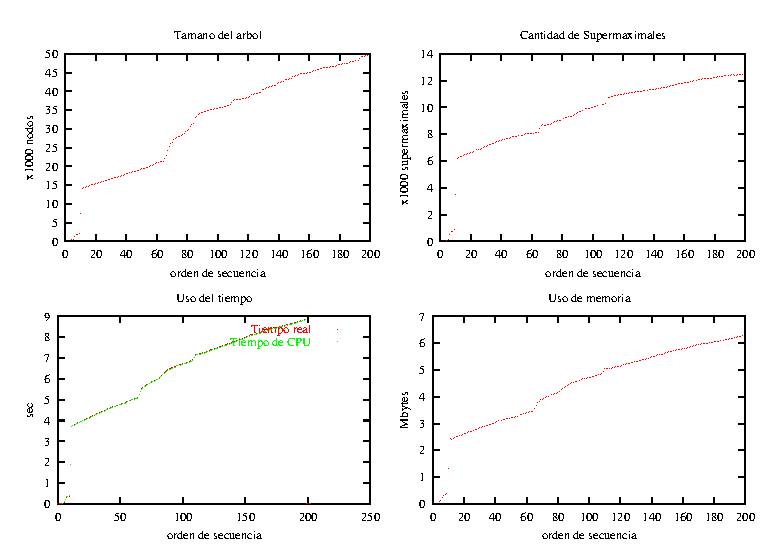
\includegraphics{Tcg.vipersire.5.eps}} \par}
\caption[Resultados. Secuencias \emph{Trypanosoma cruzi} con SIRE y VIPER (5x).]{\label{Figure:tcg.SIRE/VIPER.5x}Resultados. Secuencias \emph{Trypanosoma cruzi} con secuencias SIRE y VIPER. Cobertura 5x.}
\end{figure}

\begin{figure}
{\centering \resizebox*{1\columnwidth}{!}{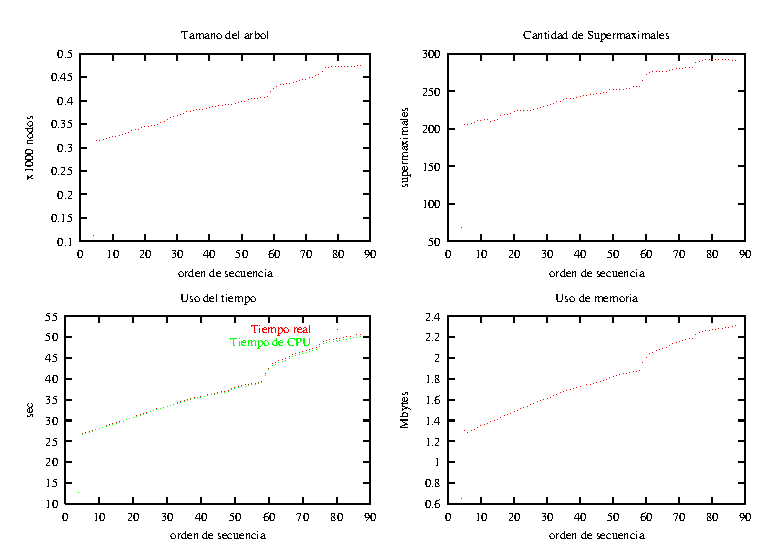
\includegraphics{Tcg.vipersire.195.eps}} \par}
\caption[Resultados. Secuencias \emph{Trypanosoma cruzi} con SIRE y VIPER (195x).]{\label{Figure:tcg.SIRE/VIPER.195x}Resultados. Secuencias \emph{Trypanosoma cruzi} con secuencias SIRE y VIPER. Cobertura 195x.}
\end{figure}

\subsubsection{BAC ends}

\begin{description}
\item [Origen~de~las~secuencias]Entrez. Secuencias BAC ends. Las librer�as BAC se componen de fragmentos de largos mayores a 100Kb. Se usan en secuenciamientos aleatorios jer�rquicos. Es otra etapa del secuenciamiento donde es interesante observar la distribuci�n de las repeticiones, ya que una gran cantidad de estas en esta etapa puede contraer grandes complicaciones en el ensamblado. En la actualidad este proceso se realiza con t�cnicas bioqu�micas como \emph{fingerprinting} para descartar los BACs que est�n con estos elementos. Ver "TIGR Sequencing Strategy for \emph{T. cruzi}" en \\ \emph{http://www.tigr.org/tdb/mdb/tcdb/seq.shtml}.\\Consulta en Entrez:
\begin{verbatim}
("Trypanosoma cruzi"[Organism] AND BAC[All Fields])
\end{verbatim}
\item [Cantidad~de~secuencias]14450.
\item [Cobertura]14. Este n�mero es demostrativo.
\end{description}

\begin{figure}
{\centering \resizebox*{1\columnwidth}{!}{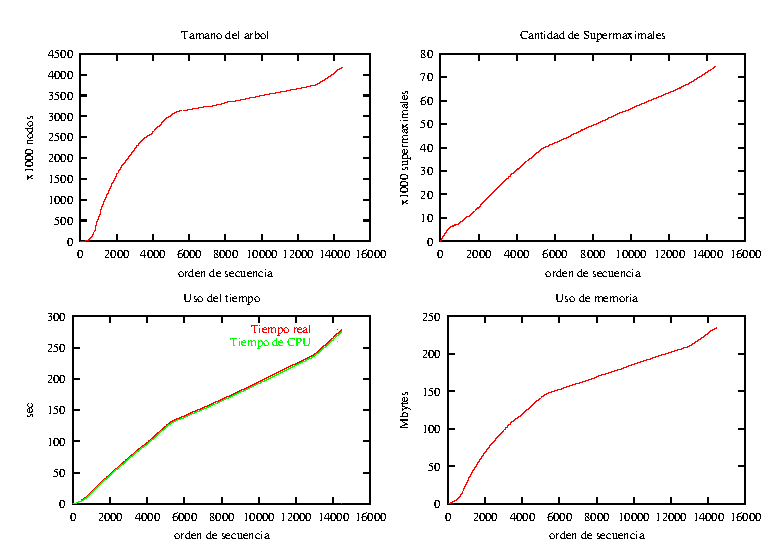
\includegraphics{Tcg.eps}} \par}
\caption[Resultados. Secuencias BAC ends del \emph{Trypanosoma cruzi}.]{\label{Figure:tcg.BACend}Resultados. Secuencias BAC ends del proyecto genoma del \emph{Trypanosoma cruzi}, clon CL-Brener.}
\end{figure}

\subsection{\emph{Plasmodium falciparum}}

\subsubsection{Secuencias de primera lectura}
\begin{description}
\item [Origen~de~las~secuencias]TIGR. Secuenciamiento WCS sobre el cromosoma 2 del \emph{Plasmodium falciparum} con una cobertura de 10x.
\item [Cantidad~de~secuencias]21807
\item [Cobertura]20. Para encontrar �nicamente repeticiones en un conjunto de secuencias cuya cobertura es 10x, se decidi� acotar en 20 la cobertura del algoritmo.
\end{description}

\begin{figure}
{\centering \resizebox*{1\columnwidth}{!}{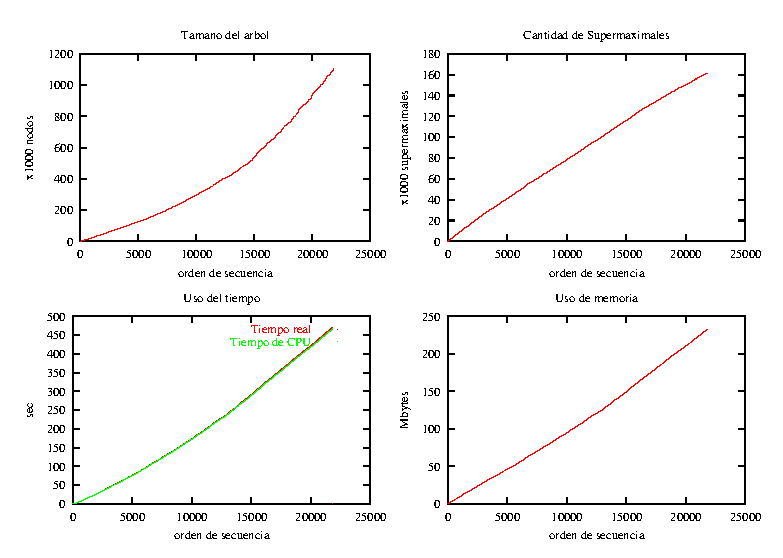
\includegraphics{Pfg.eps}} \par}
\caption[Resultados. \emph{Plasmodium falciparum}.]{\label{Figure:pfg}Resultados. \emph{Plasmodium falciparum}.}
\end{figure}

\subsubsection{Cromosoma 2 completo}
\begin{description}
\item [Origen~de~las~secuencias]TIGR. Consenso del cromosoma 2 del \emph{Plasmodium falciparum}.
\item [Cantidad~de~secuencias]1
\item [Cobertura]2. Como solo es una �nica secuencia, se tomo el valor 2 para encontrar todos las repeticiones exactas existentes en el cromosoma.
\end{description}

Luego de realizar una serie de experimentos con dichos algoritmos se ha observado la linealidad de los algoritmos. Se puede ver a continuaci�n la lista de las pruebas con sus respectivos resultados. En el caso que la cantidad de nodos el �rbol sea inferior a 100 podr� observarse tambi�n un gr�fico del mismo. Se adjunta tambi�n comparaciones gr�ficas sobre el crecimiento de los nodos, cantidad de supermaximales, cantidad sufijos de supermaximales, memoria usada y tiempo de la inserci�n.

\begin{table}
\begin{tabular}{|c||c|c|c|c|}
\hline
Muestras&tcruzi&tcruzi&pfg chr2&pfg chr2\\
&VIPER/SIRE&BAC end&WGS&Completo\\
\hline
\hline
Secuencias&195&14450&21807&1\\
\hline
Cobertura&5&14&20&2\\
\hline
Tiempo (seg)&8,85&278,42&470,79&2819,31\\
\hline
Repeticiones&12476&74692&161619&32376\\
\hline
Nodos&49665&4,17x$10^9$&1,10x$10^9$&99x$10^6$\\
\hline
Memoria (Mb)&6,6&235,01&232,86&29,56\\
\hline
\hline
\end{tabular}
\vspace{.5cm}

\caption{\label{tab:ResumenMuestras}Resumen estad�stico de las muestras seleccionadas.}
\end{table}

\section{\label{Conclusiones}Conclusiones}


\subsection{�rboles de sufijos de supermaximales.}

Mantener una estructura de un �rbol de sufijos es muy dif�cil por
el orden de almacenamiento que se necesita para una base de datos
que se incremente diariamente con secuencias muy largas. Para almacenar
el secuenciamiento de un genoma de \( s \) pb, con una cobertura
de \( c \), con la tecnolog�a actual que nos permita obtener lecturas
de promedio \( l \), el �rbol de sufijos necesita almacenar \( c\frac{s}{l} \)
fragmentos de un largo \( l \). Con lo que nos queda que el �rbol
debe tener \( c\frac{s}{l}\frac{l(l+1)}{2}=c\frac{s(l+1)}{2} \)nodos.
En un genoma como del \emph{T. cruzi}, que tiene un tama�o aproximado
de \( 87.10^{6} \)pb, con una cobertura de 10, tenemos que necesitamos
\( 28318,5.10^{7} \). Si cada nodo se podr�a almacenar en un byte,
necesitar�amos de \( 2.10^{11} \)bytes, aproximadamente \( 18 \)Gb.


\subsection{Sobre el �lgebra de repeticiones.}

En s�, el �lgebra de repeticiones no da propiedades sobre las repeticiones.
Solo fue definido para demostrar la validez del algoritmo. A�n as�
se han encontradas m�s propiedades que no son de utilidad para esta
tesis, pero si que pueden ser de inter�s para futuros algoritmos sobre
estos elementos.


\subsection{Sobre el algoritmo y su implementaci�n.}

La principal ventaja de este algoritmo no es la velocidad en que puede
calcular todas las repeticiones maximales, sino la posibilidad de
consultar dichas en cualquier momento del proceso de inserci�n, con
lo que no es necesario tener terminado el proceso de inserci�n (secuenciamiento)
para conocer todas las repeticiones. As� se puede encarar inteligentemente
el ensamblado de la secuencia principal, eliminando de antemano secuencias
que sabemos que van provocar ambig�edades.

Es un detalle m�s que importante el uso de un �rbol de sufijos como
base de la estructura de datos. La cantidad de algoritmo de consultas
de orden lineal que existen sobre dicha estructura da una potencia
extra a la misma. Algunos de estos algoritmos son: alineamiento local,
semi-global y global, b�squeda de pal�ndromos, etc.

A�n as�, su uso esta limitado a la cantidad de memoria necesaria para
procesar dicha informaci�n. Se espera poder implementar la estructura
en disco para aumentar su capacidad, como tambi�n para reducir el
efecto producido por el intercambio de p�ginas de memoria.


\subsection{Sobre la cantidad de repeticiones supermaximales.}

La cantidad de repeticiones supermaximales exactas se hace muy complicado
realizar un estudio serio sobre las repeticiones de un conjunto grande
de secuencias. Por eso se recomienda el uso de visualizaci�n cient�fica
y data-mining que simplifiquen la tarea de obtener conclusiones sobre
las secuencias.


\paragraph{Orden de importancia de secuencias.}

�Son importantes todas las secuencias repetidas supermaximales? La
respuesta a esta pregunta es completamente subjetiva, por lo tanto
dar una medida de importancia un�nime es completamente irresponsable.
A�n as� se puede realizar un estudio estad�stico sobre ellas viendo
su complejidad, largo y cantidad de copias encontradas como primer
punta del ovillo.


\paragraph{Visualizaci�n.}

La herramienta ideal para interpretar la gran cantidad de resultados
de manera global es un gr�fico. Existen varias formas de representar
las secuencias repetidas y aqu� trataremos de dar un par de ideas
nuevas para su mejor interpretaci�n.

\begin{itemize}
\item Grafos: Los grafos son una excelente manera de describir la composici�n
de las repeticiones. Por ello, si es necesario estudiar la estructura
de las secuencias, no hay mejor herramienta. La limitaci�n mayor esta
dada por la complejidad de los algoritmos sobre grafos que ayuden
a realizar conclusiones sobre los mismos.

\begin{itemize}
\item Secuencias relacionadas por supermaximales: Este grafo se basa en
relacionar secuencias seg�n los maximales que incluyen. Si visualizamos
el grafo tratando de acercar a los nodos que m�s ejes tienen en com�n
podremos visualizar nichos de secuencias donde las mismas est�n compuestas
por una repetici�n/es m�s compleja/s. El defecto principal sobre este
grafo es la cantidad de nodos que usa dicho grafo, igual a la cantidad
de secuencias de nuestro conjunto.
\item Supermaximales relacionadas por secuencias: En vez de relacionar secuencias,
ahora se relacionan supermaximales por secuencias. Esto solo reduce
la cantidad de nodos, pero todav�a sigue siendo dif�cil de manejar
ya que la cantidad de ejes pasa a ser por lo menos la cantidad de
secuencias de nuestro conjunto.

\begin{itemize}
\item Orden de repeticiones: Una manera de ver la organizaci�n de las secuencias
repetidas es ordenar las repeticiones seg�n su ubicaci�n dentro de
las secuencias que las componen. Reduce la complejidad del grafo,
a�n as� en conjuntos grandes se hace dif�cil de representar.
\item Orden de repeticiones sin relaciones transitivas: El grafo descripto
anteriormente puede reducirse elimin�ndose los ejes transitivos. El
defecto de este grafo es la complejidad del algoritmo para eliminar
dichos ejes. Notar que no existen ciclos si tomamos como ciclo a aquellos
caminos que repiten la misma copia de una repetici�n para una misa
secuencia.
\end{itemize}
\end{itemize}
\item Distribuci�n de repeticiones sobre una secuencia: En vez de representar
todas las secuencias en un �nico gr�fico, puede visualizarse la distribuci�n
de las repeticiones por secuencia. La principal desventaja es la cantidad
de secuencias que tiene el conjunto, por lo tanto se hace in�til obtener
todas las secuencias representadas.
\end{itemize}

\paragraph{Navegaci�n.}

En vez de tener un dibujo del resultado, se puede navegar permitiendo mostrar el resultado seg�n la importancia que se quiera dar al problema. Nuevamente, hay que tener un punto de donde partir a buscar conclusiones, dar un orden de importancia a las secuencias se hace indispensable.

\begin{itemize}
\item Navegaci�n basada en secuencias: Cambiar de secuencia gracias a la relaci�n de secuencias por repeticiones comunes. El resultado es un grafo de secuencias relacionadas por repeticiones, pero filtrado por el usuario.
\item Navegaci�n basada en repeticiones: Seg�n una repetici�n se puede relacionar con otra repetici�n seg�n las secuencias que las contienen. El resultado es un grafo de repeticiones relacionadas por secuencias, pero filtrado por el usuario.

\begin{itemize}
\item A partir de un conjunto seleccionable de secuencias: En vez de obtener
las repeticiones maximales a partir del conjunto completo, se puede
elegir un conjunto de secuencias y obtener cualquiera de los grafos
descripto. Luego, eliminar o agregar secuencias hasta obtener un grafo
deseado.
\end{itemize}
\end{itemize}

\paragraph{Reformular el concepto de secuencias supermaximales.}

El concepto propuesto de repetici�n no es suficientemente para un
conjunto grande de secuencia. Adem�s tiene un gran defecto, enmascara
repeticiones que pueden tener un potencial muy grande para su estudio.
Tomemos el caso de las islas CG; por la definici�n de repetici�n supermaximal,
esta secuencia no es supermaximal si existe una secuencia maximal
si la contiene, por lo tanto cualquier secuencia maximal que incluya
la cadena CG hace que la repetici�n no sobresalga a la luz. Este problema
puede resolverse con repeticiones inexactas o ampliando el concepto
de secuencias supermaximales donde la cota de cantidad de copias no
este dado por un n�mero fijo, sino por un valor relativo. Por ejemplo,
es maximal si se reduce por lo menos \( \frac{1}{3} \) la cantidad
de copias si se le agrega un nuevo car�cter.


\subsection{Resumen de las contribuciones.}

\begin{description}
\item [�lgebra~de~subsecuencias]Existen propiedades del �lgebra propuesta que no se ha desarrollado por salir del objetivo de la tesis, pero da un punto de vista interesante al tratamiento de elementos repetidos. En primer lugar puede ser la punta para desarrollar un lenguaje de consulta de este tipo de elementos, pero para ello primero se debe agregar m�s potencia de expresividad para incorporar, por ejemplo, repeticiones en t�ndem y repeticiones inexactas. Tambi�n permitir�a clasificar secuencias de forma un�voca. En si, es una herramienta nueva con mucho potencial en el �rea del estudio de repeticiones, como tambi�n en el desarrollo de algoritmos para su detecci�n.
\item [Nuevo~modelo~de~repeticiones~supermaximales]El modelo de repeticiones supermaximales en un conjunto de secuencias dependientes no fue planteado previamente. Creada en principio para resolver problemas relacionados con la gen�mica, al ser planteado para cualquier lenguaje, puede ser aplicada para la b�squeda de patrones en cualquier modelo donde exista un conjunto de muestras superpuestas hasta cierto grado de cobertura. Un ejemplo ser�a encontrar frases repetidas en un conjunto de trozos de hojas que provienen de copias de un mismo libro.
\item [�rboles~de~sufijo~de~repeticiones~supermaximales]La estructura $AS^2$\\solo se especializa en supermaximales, con lo que no cae en la sobreinformaci�n, y por basarse en una estructura muy estudiada como son los �rboles de sufijo, se conoce muy bien sus propiedades.
\item [Algoritmo~para~reconocer~repeticiones]La aplicaci�n que se le ha dado a la teor�a desarrollada corresponde al secuenciamiento de genomas bajo una t�cnica de secuenciamiento aleatorio. El algoritmo desarrollado permite que durante todo este proceso, que dura a�os, pueda mantenerse una base de datos actualizada continuamente con la informaci�n de todas las secuencias repetidas del genoma seg�n pase el tiempo. La consulta es inmediata y valida hasta ese momento, permitiendo seleccionar mejor las secuencias a ensamblar previniendo los problemas ya descriptos. Tambi�n es una herramienta muy valiosa para quienes investigan estos elementos, ya que da una pauta de la cantidad y calidad de elementos repetidos existentes
en el genoma.
\end{description}

\subsection{Investigaci�n futura.}

\begin{description}
\item [Implementaci�n~de~persistencia]La implementaci�n usa la memoria principal para almacenar la estructura $AS^2$. Aunque se conoce que puede usarse el disco, aprovechando mejor la memoria principal y no llegar al problema de intercambio de p�ginas, no ha sido como objetivo de la tesis dicha implementaci�n.  Tambi�n es de inter�s ver el comportamiento de la misma bajo un sistema concurrente, ya que en secuenciamientos a gran escala, donde m�s de cien m�quinas aportan lecturas aleatorias durante todo el d�a, es necesario atender y organizar la mayor cantidad de informaci�n en el tiempo m�s corto posible.
\item [B�squeda~inexacta~de~repeticiones]Como se ha descripto en la introducci�n, las repeticiones tienen regiones m�s y menos conservadas. El algoritmo propuesto solo busca regiones conservadas, sin t�rminos medios, con lo que no se encuentras repeticiones en el concepto biol�gico. Es de inter�s agrandar el modelo a repeticiones inexactas para mejorar la calidad de la respuesta.
\item [Nuevos~modelos~de~repeticiones~supermaximales]Como hemos visto, el concepto de maximal depend�a de la inserci�n de un nuevo car�cter. Aqu� hemos agregado el concepto de cota en cantidad de copias. Ser�a de inter�s agregar un conceptos relativos, como por ejemplo el de porcentaje de copias con respecto a su largo.
\item [Interpretaci�n~de~los~resultados] En esta tesis no se plante� observaciones sobre los elementos para poder caracterizarlos seg�n su estructura. Es de inter�s poder clasificar de forma inteligente y un�voca estos elementos para su mejor estudio.
\item [Visualizaci�n~de~los~resultados]La cantidad de soluciones es extraordinaria. Un resultado interesante en el mar de supermaximales es casi imperceptible, incapaz de resaltar sobre los dem�s. Pero de la misma manera en que se puede observar grandes movimientos de aguas bajo la superficie del mar a grandes alturas, es necesario ver las diferentes formas en que se expresan estos elementos entre ellos. Por ello se propone realizar un intenso estudio sobre la visualizaci�n de los elementos para resaltar relaciones y propiedades que son imposibles de ver con solo conocer la secuencia.
\item [Reensamblar~subsecuencias~de~repeticiones]Existen t�cnicas para recuperar la historia de replicaci�n de ADN \cite{Fitch86}. A partir de este hecho podemos realizar dos preguntas que podr�an resolver el problema de reensamblar subsecuencias de repeticiones: �Si se puede deducir dos historias parecidas de dos repeticiones, se puede deducir que pertenecen a la misma repetici�n? �La t�cnica propuesta por \cite{Fitch86} es �til con fragmentos de repeticiones? Tambi�n podemos preguntarnos que ocurre con la distribuci�n y complejidad de estos elementos para saber si estos tambi�n son posible de relacionar. Hay un campo muy grande por donde investigar que puede ayudar a deducir repeticiones de gran tama�o, m�s grande de lo que soporta el secuenciado, y as� resolver el problema de ambig�edad del ensamblado.
\end{description}


\bibliographystyle{plain}
\bibliography{Tesis}

\end{document}
